% !TeX program = xelatex
% Biên dịch: latexmk -xelatex main.tex.
\documentclass[12pt,a4paper,oneside]{report}
\usepackage{fontspec}
\usepackage{polyglossia}
\setdefaultlanguage{vietnamese}
\setotherlanguage{english}
\setmainfont{Times New Roman}
\usepackage{geometry}
\geometry{left=3.0cm,right=2.5cm,top=2.0cm,bottom=2.0cm,headheight=14pt,headsep=0.4cm,footskip=1.0cm}
\usepackage{amsmath,amssymb,booktabs,longtable,array,graphicx,caption,hyperref,xcolor,float,enumitem,fancyhdr}
\usepackage{titlesec,tocloft,tikz}
\usepackage{indentfirst}
\hypersetup{colorlinks=true,linkcolor=black,urlcolor=blue,citecolor=black}
\makeatletter
\renewcommand{\normalsize}{\@setfontsize\normalsize{13pt}{19.5pt}}
\makeatother
\AtBeginDocument{\normalsize}
\setlength{\parindent}{1.25cm}
\setlength{\parskip}{0pt}
\setlength{\emergencystretch}{2em}
\clubpenalty=10000
\widowpenalty=10000
\displaywidowpenalty=10000
\renewcommand{\contentsname}{MỤC LỤC}
\renewcommand{\listfigurename}{DANH MỤC HÌNH ẢNH}
\renewcommand{\listtablename}{DANH MỤC CÁC BẢNG}
\renewcommand{\figurename}{Hình}
\renewcommand{\tablename}{Bảng}
\renewcommand{\bibname}{TÀI LIỆU THAM KHẢO}
\titleformat{\chapter}[block]
  {\normalfont\bfseries\centering\fontsize{14pt}{18pt}\selectfont}
  {\MakeUppercase{\chaptertitlename}~\thechapter:}
  {0.5em}
  {\MakeUppercase}
\titlespacing*{\chapter}{0pt}{18pt}{4pt}
\titleformat{\section}
  {\normalfont\bfseries\fontsize{16pt}{20pt}\selectfont}
  {\thesection.}{0.5em}{}
\titlespacing*{\section}{0pt}{1.5ex plus 0.4ex minus 0.2ex}{0.8ex}
\titleformat{\subsection}
  {\normalfont\bfseries\fontsize{14pt}{18pt}\selectfont}
  {\thesubsection.}{0.5em}{}
\titlespacing*{\subsection}{0pt}{1.3ex plus 0.3ex minus 0.2ex}{0.6ex}
\titleformat{\subsubsection}
  {\normalfont\bfseries\fontsize{13pt}{16pt}\selectfont}
  {\thesubsubsection.}{0.5em}{}
\titlespacing*{\subsubsection}{0pt}{1.1ex plus 0.2ex minus 0.2ex}{0.5ex}
\setcounter{tocdepth}{2}
\renewcommand{\cftchapleader}{\cftdotfill{\cftdotsep}}
\setlength{\cftbeforechapskip}{0.35em}
\setlength{\cftchapnumwidth}{2.8em}
\setlength{\cftsecindent}{1.8em}
\setlength{\cftsecnumwidth}{3.4em}
\setlength{\cftsubsecindent}{5.2em}
\setlength{\cftsubsecnumwidth}{3.6em}
\renewcommand{\cfttoctitlefont}{\hfill\normalfont\bfseries\fontsize{14pt}{18pt}\selectfont}
\renewcommand{\cftaftertoctitle}{\hfill}
\renewcommand{\cftlottitlefont}{\hfill\normalfont\bfseries\fontsize{14pt}{18pt}\selectfont}
\renewcommand{\cftafterlottitle}{\hfill}
\renewcommand{\cftloftitlefont}{\hfill\normalfont\bfseries\fontsize{14pt}{18pt}\selectfont}
\renewcommand{\cftafterloftitle}{\hfill}
\captionsetup{font=small,labelfont=bf,justification=centering,singlelinecheck=false}
\pagestyle{fancy}
\fancyhf{}
\fancyhead[C]{\fontsize{11pt}{13pt}\selectfont\bfseries Phát hiện vật cản trong ảnh hỗ trợ người khiếm thị}
\fancyfoot[C]{\fontsize{11pt}{13pt}\selectfont\thepage}
\renewcommand{\headrulewidth}{0.4pt}
\fancypagestyle{plain}{%
  \fancyhf{}
  \fancyhead[C]{\fontsize{11pt}{13pt}\selectfont\bfseries Phát hiện vật cản trong ảnh hỗ trợ người khiếm thị}
  \fancyfoot[C]{\fontsize{11pt}{13pt}\selectfont\thepage}
  \renewcommand{\headrulewidth}{0.4pt}
}
\begin{document}
\renewcommand{\contentsname}{MỤC LỤC}
\renewcommand{\listfigurename}{DANH MỤC HÌNH ẢNH}
\renewcommand{\listtablename}{DANH MỤC CÁC BẢNG}

\begin{titlepage}
\thispagestyle{empty}
\begin{tikzpicture}[remember picture,overlay]
  \draw[line width=0.8pt]
    ([xshift=1.4cm,yshift=-1.4cm]current page.north west)
    rectangle
    ([xshift=-1.4cm,yshift=1.4cm]current page.south east);
\end{tikzpicture}
\vspace*{0.25cm}
\centering
{\large\bfseries BỘ GIÁO DỤC VÀ ĐÀO TẠO\par}
\vspace{0.15cm}
{\large\bfseries TRƯỜNG ĐẠI HỌC CÔNG NGHỆ KỸ THUẬT HƯNG YÊN\par}
\vspace{0.45cm}
\IfFileExists{logo_truong.jpg}{\includegraphics[width=2.1cm]{logo_truong.jpg}}{\fbox{\parbox[c][1.8cm][c]{2.1cm}{\centering LOGO TRƯỜNG}}}\par
\vspace{0.35cm}
\rule{5.8cm}{0.6pt}\par
\vspace{1.05cm}
{\Large\bfseries BÀI TẬP LỚN\par}
{\Large\bfseries HỌC SÂU\par}
\vspace{0.75cm}
{\large\bfseries
  \parbox{0.88\textwidth}{\centering
    PHÁT HIỆN VẬT CẢN TRONG ẢNH\\
    HƯỚNG TỚI HỖ TRỢ DI CHUYỂN\\
    CHO NGƯỜI KHIẾM THỊ\par}}\par
\vspace{0.6cm}
{\normalsize NGÀNH: KHOA HỌC MÁY TÍNH\par}
{\normalsize CHUYÊN NGÀNH: TRÍ TUỆ NHÂN TẠO VÀ KHOA HỌC DỮ LIỆU\par}
\vfill
{\normalsize
Sinh viên: \textbf{NGUYỄN TRẦN KIÊN}\par
Mã sinh viên: \textbf{12423018}\par
Mã lớp: \textbf{12423TN}\par
Giảng viên hướng dẫn: \textbf{PGS.TS. NGUYỄN MINH TIẾN}\par}
\vfill
{\large\bfseries HƯNG YÊN -- 2026\par}
\end{titlepage}
\setcounter{page}{2}

\chapter*{NHẬN XÉT}
\addcontentsline{toc}{chapter}{NHẬN XÉT}
\noindent Nhận xét của giảng viên hướng dẫn:\par
\newcommand{\reviewline}{\noindent\makebox[\textwidth]{\dotfill}\par\vspace{0.35cm}}
\reviewline\reviewline\reviewline\reviewline\reviewline
\reviewline\reviewline\reviewline\reviewline\reviewline
\reviewline\reviewline\reviewline\reviewline\reviewline
\begin{flushright}\textbf{GIẢNG VIÊN HƯỚNG DẪN}\\[1.8cm]
\textbf{PGS.TS. Nguyễn Minh Tiến}\end{flushright}

\chapter*{LỜI CAM ĐOAN}
\addcontentsline{toc}{chapter}{LỜI CAM ĐOAN}
Em xin cam đoan dự án “PHÁT HIỆN VẬT CẢN TRONG ẢNH HƯỚNG TỚI HỖ TRỢ DI CHUYỂN CHO NGƯỜI KHIẾM THỊ” là kết quả thực hiện của bản thân em dưới sự hướng dẫn của thầy Nguyễn Minh Tiến.

Các tài liệu tham khảo sử dụng trong đồ án đã được nêu rõ trong phần tài liệu tham khảo. Các kết quả trình bày trong đồ án và chương trình xây dựng hoàn toàn là kết quả thực hiện của riêng em.

Nếu vi phạm cam kết này, em xin chịu hoàn toàn trách nhiệm trước khoa và nhà trường.

Hưng yên, ngày 19 tháng 06 năm 2026

Sinh viên

Kiên

Nguyễn Trần Kiên

\chapter*{LỜI CẢM ƠN}
\addcontentsline{toc}{chapter}{LỜI CẢM ƠN}
Để có thể hoàn thành đồ án này, lời đầu tiên em xin phép gửi lời cảm ơn tới bộ môn Khoa học máy tính, Khoa Công nghệ thông tin – Trường Đại học Sư phạm Kỹ thuật Hưng Yên đã tạo điều kiện thuận lợi cho em thực hiện đồ án môn học này.

Đặc biệt em xin chân thành cảm ơn thầy Nguyễn Minh Tiến đã rất tận tình hướng dẫn, chỉ bảo em trong suốt thời gian thực hiện đồ án vừa qua.

Em cũng xin chân thành cảm ơn tất cả các Thầy, các Cô trong Trường đã tận tình giảng dạy, trang bị cho em những kiến thức cần thiết, quý báu để giúp em thực hiện được đồ án này.

Mặc dù em đã có cố gắng, nhưng với trình độ còn hạn chế, trong quá trình thực hiện đề tài không tránh khỏi những thiếu sót. Em hy vọng sẽ nhận được những ý kiến nhận xét, góp ý của các Thầy cô về những kết quả triển khai trong đồ án.

Em xin trân trọng cảm ơn!

\clearpage
\tableofcontents
\clearpage
\chapter*{DANH MỤC CÁC THUẬT NGỮ}
\addcontentsline{toc}{chapter}{DANH MỤC CÁC THUẬT NGỮ}
\begin{longtable}{p{2.4cm}p{4.6cm}p{7.2cm}}
\toprule Ký hiệu & Cụm từ & Diễn giải\\\midrule
AP & Average Precision & Diện tích nội suy dưới đường Precision--Recall tại một lớp và một ngưỡng IoU.\\
COCO & Common Objects in Context & Bộ dữ liệu và hệ quy ước đánh giá phát hiện đối tượng phổ biến.\\
FPN & Feature Pyramid Network & Mạng kim tự tháp đặc trưng dùng biểu diễn nhiều tỉ lệ.\\
FN/FP/TP & False Negative/False Positive/True Positive & Bỏ sót, báo nhầm và phát hiện đúng theo quy tắc ghép.\\
IoU & Intersection over Union & Tỷ lệ diện tích giao trên diện tích hợp của hai hộp.\\
mAP & mean Average Precision & Trung bình AP qua lớp và qua nhiều ngưỡng IoU.\\
NMS & Non-Maximum Suppression & Hậu xử lý loại các hộp dự đoán trùng lặp.\\
ROD & Real-Time Obstacle Detection & Bộ dữ liệu vật cản đường phố dùng trong đồ án.\\
RPN & Region Proposal Network & Mạng đề xuất vùng trong Faster R-CNN.\\
VALID & Validation split & Tập xác thực dùng chọn checkpoint, ngưỡng và phân tích mô hình.\\
\bottomrule
\end{longtable}\clearpage
\listoftables
\clearpage
\listoffigures
\clearpage
\chapter{TỔNG QUAN VỀ ĐỀ TÀI}\label{chap:intro}
\section{Lý do chọn đề tài}
Người sử dụng ảnh cần biết vật thể nào xuất hiện và vật thể đó nằm ở đâu. Bài toán phát hiện đối tượng vì vậy yêu cầu dự đoán đồng thời một hình chữ nhật bao quanh vật thể, tên lớp và điểm tin cậy. Điểm tin cậy là đầu ra của mô hình; nó không phải xác suất an toàn đã được hiệu chuẩn. Từ góc nhìn ứng dụng hỗ trợ, bỏ sót một vật cản quan trọng có thể gây hậu quả hơn một cảnh báo sai, nhưng kết luận về an toàn thực tế đòi hỏi nghiên cứu người dùng và điều kiện sử dụng ngoài phạm vi báo cáo này.

Câu hỏi nghiên cứu là: (i) thay YOLO11n bằng YOLO11s có cải thiện Recall và chất lượng định vị đủ để đánh đổi độ trễ và kích thước hay không; (ii) Faster R-CNN có mang lại lợi ích phát hiện tương ứng với chi phí suy luận hay không; (iii) ba mô hình có thể vận hành trong ứng dụng xử lý ảnh tải lên ở mức độ nào. Mô hình lớn hơn có thể học biểu diễn phong phú hơn, nhưng điều đó không bảo đảm mọi lớp đều tốt hơn hoặc độ trễ phù hợp phần cứng hạn chế. Giả thuyết được khảo sát bằng VALID trong giai đoạn phát triển và được kiểm tra cuối bằng TEST đã khóa tại Chương~\ref{chap:results}.

Sản phẩm hiện hành chỉ xử lý ảnh tĩnh: tải ảnh, chọn mô hình, phát hiện, hiển thị hộp bao, nhãn, confidence, thống kê và tải ảnh kết quả.  Không có webcam, ước lượng khoảng cách, cảnh báo âm thanh, GPS hay dẫn đường; ứng dụng không thay thế phương tiện hỗ trợ di chuyển chuyên dụng.

Sự khác nhau giữa ảnh tĩnh và hỗ trợ di chuyển cần được giữ rõ trong cách diễn giải. Detector chỉ quan sát pixel của một thời điểm; hộp nằm gần đáy ảnh không đủ để kết luận vật thể nằm trên lối đi, và một chiếc xe ở xa có thể không phải vật cản tức thời. Độ sâu đơn ảnh, tracking và kết hợp cảm biến có thể bổ sung ngữ cảnh nhưng đều nằm ngoài hệ thống này. Phạm vi nghiên cứu vì vậy giới hạn vào năng lực nhận diện và định vị 2D, để tránh gắn một metric benchmark với tuyên bố về an toàn.

\section{Mục tiêu của đề tài}
Mục tiêu thứ nhất là xây dựng bộ dữ liệu sử dụng được cho huấn luyện và đánh giá, giữ đủ 25 lớp nhưng giảm rò rỉ giữa TRAIN, VALID và TEST. Mục tiêu thứ hai là tinh chỉnh ba detector có kiến trúc và quy mô khác nhau trong ngân sách 10 epoch hiện có. Mục tiêu thứ ba là đưa mọi checkpoint qua một evaluator chung để tránh so trực tiếp metric của hai framework. Mục tiêu cuối là tích hợp cả ba vào ứng dụng ảnh tĩnh và đo riêng thời gian suy luận với thời gian xử lý callback.

Đóng góp của đồ án nằm ở tính truy vết. Mỗi kết luận định lượng có tệp nguồn; checkpoint và ngưỡng có SHA256; TEST được khóa tới bước đánh giá cuối. Cách làm này giảm nguy cơ công bố nhầm số, dùng TEST để tinh chỉnh hoặc quy kết sai nguyên nhân. Báo cáo cũng chỉ ra khoảng trống bằng chứng của E6 và không biến code cấu hình thành lịch sử thực thi đã được kiểm chứng.

\section{Giới hạn và phạm vi của đề tài}
\subsection{Đối tượng nghiên cứu}
Đối tượng nghiên cứu là phát hiện đối tượng hai chiều trên ảnh đơn. Phạm vi dữ liệu là ROD Final A4 với 25 lớp. Phạm vi mô hình gồm E3 YOLO11n, E4 YOLO11s và E6 Faster R-CNN, đều khởi tạo từ trọng số pretrained. E6 được hiện thực bằng biến thể Faster R-CNN có backbone ResNet-50 FPN V2; tên mô hình trình bày trong báo cáo được thống nhất là Faster R-CNN. VALID chỉ dùng cho phát triển, chọn checkpoint và ngưỡng; TEST đã được chạy đúng một lượt sau khi khóa toàn bộ cấu hình để báo cáo kết quả cuối.

\subsection{Phạm vi nghiên cứu}
Báo cáo không đánh giá khoảng cách, quỹ đạo, độ sâu đơn ảnh, giọng nói, định vị, khả năng sử dụng của người khiếm thị hoặc độ an toàn ngoài đời. Các chương sau trình bày dữ liệu, lý thuyết, thiết kế thực nghiệm, kết quả, ứng dụng và giới hạn theo thứ tự đó.


\section{Nội dung thực hiện}
Công việc bắt đầu bằng khảo sát ROD nguồn, kiểm tra cấu trúc thư mục, taxonomy, annotation và thống kê object. Các vòng làm sạch loại bỏ ảnh/nhãn lỗi theo manifest, rà soát trùng lặp, phân tích rò rỉ và đóng băng Final A4. Kế tiếp, nhãn được chuẩn hóa cho hai framework; cấu hình fine-tune được thiết lập; checkpoint được lưu; ngưỡng được lựa chọn bằng VALID; metric được tính lại trong evaluator chung. Cuối cùng, benchmark tách latency inference và callback, rồi ba model được đưa vào giao diện Gradio cho ảnh tải lên.

Mỗi giai đoạn tạo ra bằng chứng khác nhau. Tệp cấu hình mô tả tham số dự kiến; checkpoint chứa trọng số; log cho biết tiến trình huấn luyện; cache prediction cho phép quét lại threshold; JSON evaluator lưu metric; kiểm thử phần mềm xác nhận một số hợp đồng đầu vào/đầu ra. Không thể suy đường cong huấn luyện từ checkpoint hoặc suy rằng cấu hình đã chạy chỉ vì tệp cấu hình tồn tại.

\section{Phương pháp tiếp cận}
Nghiên cứu là thực nghiệm so sánh trên split cố định. TRAIN cập nhật trọng số; VALID dùng theo dõi, chọn checkpoint và threshold; TEST chỉ dành cho đánh giá cuối sau khi mọi quyết định được khóa. Cùng protocol được áp dụng sau huấn luyện để các framework không tự định nghĩa metric xếp hạng khác nhau. Tuy nhiên, so sánh không phải ablation hoàn hảo vì kiến trúc, input transform, loss và lịch huấn luyện khác nhau.

Để tăng khả năng tái lập, báo cáo ghi mapping lớp, quy tắc matching, ngưỡng IoU, NMS, giới hạn detection, hash và điều kiện benchmark. Kết luận được giới hạn ở checkpoint và dữ liệu đã đo; các khác biệt nhỏ chưa có khoảng tin cậy hoặc nhiều seed không được diễn giải thành ưu thế tổng quát.
\chapter{CƠ SỞ LÝ THUYẾT}\label{chap:theory}
\section{Bài toán phát hiện đối tượng}
Detector nhận ảnh và trả về nhiều dự đoán gồm hộp, class ID và confidence. Số lượng vật thể không cố định; mỗi dự đoán phải vừa đúng lớp vừa định vị đủ tốt mới được ghép với nhãn thật.
\subsection{Ảnh, lớp và bounding box}
Ảnh số là lưới pixel; annotation gắn mỗi vật thể với nhãn lớp và hộp chữ nhật. Hộp bao không phải phân đoạn pixel và có thể chứa nền. Taxonomy cùng thứ tự class ID phải thống nhất xuyên suốt dữ liệu, model, evaluator và giao diện.
\subsection{Hệ tọa độ YOLO và xyxy}
YOLO lưu tâm, rộng, cao chuẩn hóa; Torchvision dùng tọa độ pixel $(x_1,y_1,x_2,y_2)$. Quy đổi cần dùng đúng chiều rộng/cao ảnh; hộp phải thỏa $x_1<x_2$, $y_1<y_2$ và nằm trong biên. Nhầm hệ tọa độ tạo lỗi định vị dù model vẫn chạy.
Một hộp có thể biểu diễn bằng hai góc $(x_1,y_1,x_2,y_2)$ theo pixel hoặc bằng tâm, chiều rộng và chiều cao $(x_c,y_c,w,h)$. Nhãn YOLO của ROD chuẩn hóa bốn giá trị sau theo kích thước ảnh. Khi đánh giá, hệ thống chuyển về pixel để tính giao và hợp. Quá trình chuyển phải clip sai số số thực rất nhỏ ở biên nhưng không được chấp nhận hộp rỗng hoặc class ngoài 0--24.

IoU không phản ánh khoảng cách tuyệt đối giữa hai hộp. Với vật nhỏ, lệch vài pixel có thể làm IoU giảm mạnh; với vật lớn, cùng độ lệch có ảnh hưởng nhỏ hơn. Do đó mAP50 đánh giá dễ hơn mAP50--95. Khoảng cách giữa hai chỉ số giúp quan sát chất lượng định vị: model có thể tìm đúng vật thể ở IoU 0,5 nhưng hộp chưa đủ sát để giữ AP ở 0,75--0,95.

Ví dụ một GT có diện tích 10.000 pixel vuông và hộp dự đoán giao 8.000, phần ngoài giao của hai hộp tổng 4.000, khi đó hợp là 12.000 và IoU bằng 0,667. Prediction được tính đúng ở IoU 0,5 nhưng sai ở 0,7. mAP50--95 vì thế khắt khe hơn và được dùng làm tiêu chí best của các pipeline huấn luyện.
\subsection{Intersection over Union}
Một dự đoán chỉ hữu ích khi vừa đúng lớp vừa phủ đủ vật thể. Với hộp dự đoán $B_p$ và hộp tham chiếu $B_g$, mức giao nhau trên hợp (intersection over union, IoU) là
\begin{equation}\operatorname{IoU}(B_p,B_g)=\frac{|B_p\cap B_g|}{|B_p\cup B_g|}.\end{equation}
Ở đây $|\cdot|$ là diện tích. Bộ đánh giá ghép một dự đoán với tối đa một nhãn thật cùng lớp theo thứ tự điểm giảm dần; dự đoán không ghép được là báo nhầm, nhãn thật không được ghép là bỏ sót.  Trên ảnh ROD có hai người sát nhau, một hộp dự đoán phủ cả hai không thể được tính thành hai phát hiện đúng. Nguyên tắc một-một giảm đếm trùng, nhưng kết quả còn phụ thuộc ngưỡng IoU và độ chính xác nhãn gốc.

\begin{figure}[htbp]\centering
\fbox{\begin{minipage}{0.87\linewidth}\centering
Ảnh ROD $\longrightarrow$ hộp và điểm tin cậy $\longrightarrow$ ghép cùng lớp theo IoU\\
$\longrightarrow$ đúng / báo nhầm / bỏ sót $\longrightarrow$ đường cong Precision--Recall
\end{minipage}}
\caption{Luồng đánh giá chung; sơ đồ khái niệm, không phải ảnh kết quả thực nghiệm.}\end{figure}
\subsection{Ghép dự đoán với ground truth}
Quy tắc một-một ghép mỗi prediction với nhiều nhất một ground truth cùng lớp chưa dùng. Hộp không đạt IoU hoặc sai lớp trở thành FP; nhãn chưa ghép là FN. Một hộp phủ hai người không thể được đếm hai TP. Kết quả phụ thuộc thứ tự score, ngưỡng IoU và NMS.

\paragraph{Chi tiết về hình học và ghép hộp.}
Hộp bao là xấp xỉ tiện lợi cho định vị, không diễn tả hình dạng chính xác của vật cản. Nếu hai vật đứng sát nhau, một hộp gộp có thể có IoU đáng kể với cả hai nhưng vẫn chỉ ghép được một ground truth. Nếu class ID sai, hộp không được tính TP dù IoU lớn. Quy tắc cùng lớp và ghép một-một vì thế bắt buộc để phân biệt lỗi phân loại, lỗi định vị và lỗi bỏ sót.

\section{Các chỉ số đánh giá}
\subsection{True Positive, False Positive và False Negative}
TP là phát hiện ghép đúng, FP là báo nhầm, FN là vật thể bị bỏ sót. Các số này cần được xem cùng threshold và tổng ground truth; bản thân chúng không cho biết nguyên nhân.
\subsection{Precision và Recall}
Gọi $TP$ là số phát hiện đúng, $FP$ là báo nhầm và $FN$ là bỏ sót. Precision $P=TP/(TP+FP)$ phản ánh tỷ lệ dự đoán đáng tin; Recall $R=TP/(TP+FN)$ phản ánh khả năng tìm đủ vật thể. Để ưu tiên Recall khi chọn ngưỡng vận hành trên VALID, dự án dùng
\begin{equation}F_2=\frac{(1+2^2)PR}{2^2P+R}.\end{equation}
Hệ số hai là trọng số trong tiêu chí lựa chọn, không biến ứng dụng thành hệ thống an toàn. Ngưỡng confidence của mỗi mô hình được chốt theo micro-$F_2$ trên VALID và không thay đổi tùy từng ảnh. 


\subsection{F1 và F2} F1 cân bằng hai chỉ số, còn F2 ưu tiên Recall:
\begin{equation}F_1=\frac{2PR}{P+R},\qquad F_2=\frac{5PR}{4P+R}.\end{equation}
Với $P=0,70$, $R=0,80$, F1 xấp xỉ 0,747 còn F2 xấp xỉ 0,778. Đây là tiêu chí chọn operating point, không phải thước đo an toàn.
\subsection{Đường Precision--Recall và Average Precision}
Khi hạ confidence threshold, model thường giữ thêm prediction: Recall tăng nhưng FP cũng có thể tăng, làm Precision giảm. Đường Precision--Recall mô tả toàn bộ đánh đổi này. Một điểm vận hành duy nhất phù hợp cho giao diện, còn AP tóm tắt thứ hạng prediction qua nhiều score. Vì thế AP không phụ thuộc đúng một threshold hiển thị, nhưng vẫn phụ thuộc prediction thu thập, NMS và giới hạn detection.

Nội suy 101 điểm lấy Precision cực đại ở Recall không thấp hơn mỗi mức $0,00;0,01;\ldots;1,00$. Phép nội suy tránh phạt các dao động cục bộ của đường cong và tạo kết quả tái lập. Nếu một lớp không có GT, cách xử lý phải được quy định; ROD Final có đủ 25 lớp trong toàn bộ dữ liệu và evaluator lưu số GT từng lớp để kiểm tra.

Micro Precision cộng TP, FP, FN của mọi lớp trước khi chia. Macro theo lớp sẽ tính từng lớp rồi trung bình. Dự án dùng micro-F2 chọn threshold vì muốn tối ưu số detection tổng thể, còn mAP trung bình đều qua lớp để không bỏ qua lớp hiếm. Hai phép tổng hợp có thể cho thứ hạng khác nhau mà không mâu thuẫn.
\subsection{mAP50 và mAP50--95}
Average precision (AP) được tính bằng diện tích rời rạc dưới đường cong Precision--Recall sau nội suy. Gọi $p^*(r)$ là Precision tốt nhất tại Recall không nhỏ hơn $r$; bộ đánh giá dùng
\begin{equation} AP_t=\frac{1}{101}\sum_{i=0}^{100}p^*_t(i/100),\qquad
 mAP_{50:95}=\frac{1}{25}\sum_{c=1}^{25}\frac{1}{10}\sum_{t\in\{0.50,0.55,\ldots,0.95\}}AP_{c,t}.\end{equation}
Chỉ số $c$ là lớp, $t$ là ngưỡng IoU. mAP50 dùng riêng $t=0.50$. AP quét nhiều mức điểm tin cậy; Precision và Recall trong bảng kết quả lại đo ở một ngưỡng vận hành. Hai loại số này trả lời hai câu hỏi khác nhau. Dự án dùng quy tắc lấy cảm hứng từ COCO \cite{coco}, nhưng mã chấm riêng không xử lý mọi trường hợp của bộ chấm COCO chính thức, do đó không gọi đây là kết quả COCO benchmark. 
\subsection{Non-Maximum Suppression}
NMS xếp hộp theo score rồi loại các hộp cùng lớp chồng lấp cao. Ngưỡng thấp có thể xóa hai vật gần nhau; ngưỡng cao có thể giữ hộp trùng. NMS và số detection là thành phần protocol, không phải chi tiết có thể thay đổi sau khi xem TEST.

\paragraph{Đọc đồng thời các chỉ số.}
Precision/Recall vận hành trả lời hiệu quả tại một threshold, còn AP phản ánh chất lượng xếp hạng trên dải score. Macro mAP cho lớp hiếm trọng số ngang lớp phổ biến, trong khi tổng TP/FP/FN phản ánh micro toàn bộ object. Hai cách tổng hợp có thể khác nhau mà không mâu thuẫn. Một mô hình có AP cao nhưng Recall thấp ở threshold thực thi vẫn cần được đánh giá theo yêu cầu ứng dụng.

\section{Các mô hình phát hiện vật thể}
\subsection{Học chuyển giao từ COCO}
COCO chứa nhiều lớp phổ biến trùng khái niệm với ROD như person, car, bus, truck và dog. Trọng số pretrained có thể cung cấp cạnh, texture, hình dạng và biểu diễn đối tượng trước khi fine-tune. Các lớp đặc thù hơn như manhole, guard rail hay electrical box cần thích nghi từ dữ liệu ROD.

Pretraining không thay thế đánh giá domain shift. Ảnh ROD có góc chụp, độ phân giải, phân bố lớp và điều kiện cảnh riêng. Ba mô hình đều pretrained nên đồ án không trả lời câu hỏi pretrained so với scratch. E5 scratch thuộc lịch sử và đã ra khỏi phạm vi; đưa E5 không hoàn chỉnh vào bảng sẽ làm sai thiết kế nghiên cứu hiện hành.
\subsection{Kiến trúc YOLO và phát hiện một giai đoạn}
YOLO dùng backbone, neck đa tỷ lệ và head để dự đoán trực tiếp vị trí/lớp. Đường suy luận gọn không đảm bảo realtime trên mọi thiết bị; tốc độ phụ thuộc resolution, backend, NMS và phần cứng.
\subsection{YOLO11n}
YOLO là họ bộ phát hiện một giai đoạn: mạng trích xuất đặc trưng ảnh rồi dự đoán trực tiếp vị trí và lớp trên nhiều tỉ lệ. Các biến thể YOLO11n và YOLO11s dùng cùng họ thiết kế, song quy mô tham số khác nhau \cite{yolo11}. Vấn đề là một vật nhỏ như biển báo có thể mất chi tiết khi giảm kích thước đặc trưng; xử lý đa tỉ lệ cho phép kết hợp thông tin rộng và chi tiết. Trong cấu hình dự án, cả hai nhận ảnh ở cùng kích thước đầu vào, còn trọng số ban đầu lần lượt là \texttt{yolo11n.pt} và \texttt{yolo11s.pt}. 

\begin{figure}[htbp]\centering
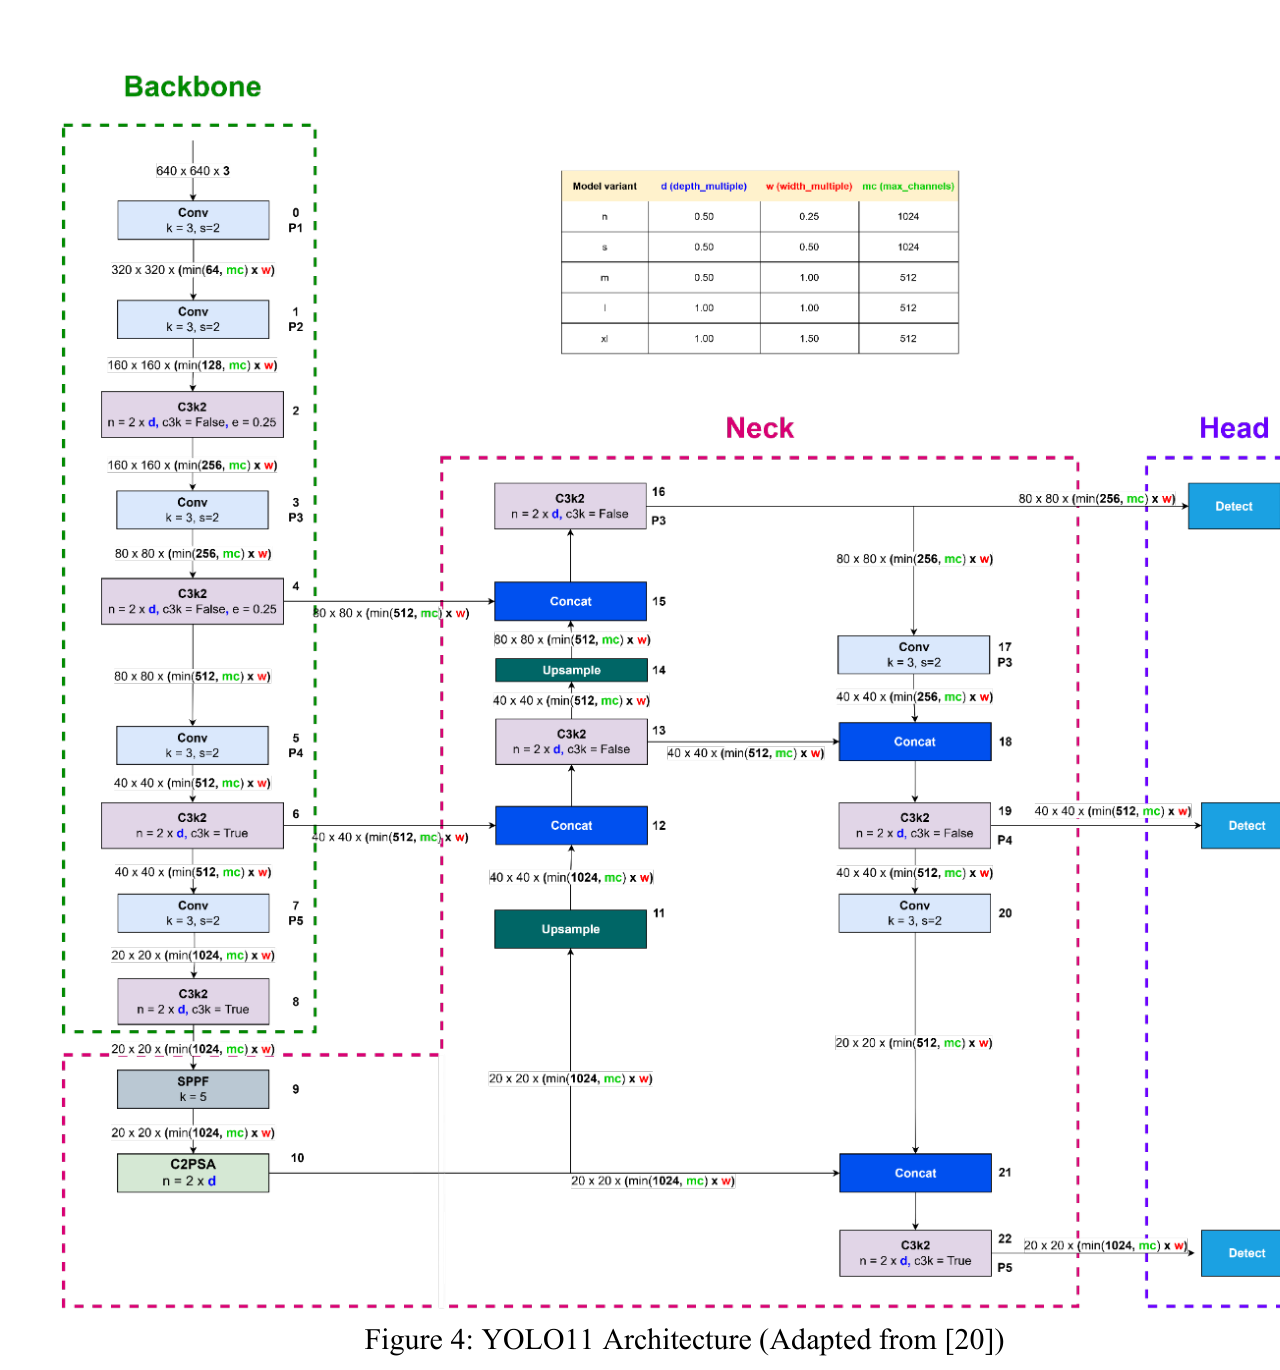
\includegraphics[width=0.98\textwidth]{figures/yolo11_architecture_original.png}
\caption{Kiến trúc YOLO11 gồm backbone, neck và detection head. Hình được trích từ Hidayatullah và cộng sự, Hình 4 trong arXiv:2501.13400 \cite{yolo11paper}; không phải sơ đồ tự vẽ.}\label{fig:yolo11architecture}
\end{figure}

Ví dụ ROD gồm người và cầu thang: mạng phải vừa giữ cấu trúc rộng của cầu thang vừa nhận các vùng người nhỏ. Ưu điểm của thiết kế một giai đoạn là đường suy luận gọn; hạn chế tiềm tàng là mô hình nhỏ có ít dung lượng biểu diễn hơn. Đây là nhận định kiến trúc, không phải bằng chứng rằng YOLO11s thắng YOLO11n trên mọi lớp. 
\subsection{YOLO11s}
Ký hiệu n và s thể hiện hai mức quy mô trong cùng họ YOLO11. Checkpoint local sau khi thay head ROD có khoảng 2,595 triệu tham số ở E3 và 9,437 triệu ở E4. Số tham số E4 gấp khoảng 3,64 lần E3; phép đo công cụ ở ảnh 640 cho 6,53 và 21,72 GFLOPs theo quy ước của Ultralytics/THOP. Các số GFLOPs chỉ so tương đối trong cùng công cụ vì operator và quy ước đếm có thể khác.

Mô hình lớn hơn có thể giữ nhiều kênh đặc trưng và học ranh giới lớp phức tạp hơn. Đổi lại, activation và phép tích chập tăng, làm latency và bộ nhớ cao hơn. Lợi ích không đồng đều theo lớp: E4 tốt hơn E3 ở nhiều lớp nhưng giảm ở Building, Electrical Pole, Motorcycle, Tree, Guard rail và Bicycle Rack trong bảng AP50--95. Một phần chênh lệch nhỏ có thể do biến thiên huấn luyện một seed.

YOLO xử lý toàn ảnh trong một mạng feed-forward và dùng đầu dự đoán dày đặc. Điều này phù hợp khi cần latency thấp. Tuy nhiên, “one-stage” không có nghĩa chỉ một layer, và “real-time” không phải thuộc tính cố định. Tốc độ phụ thuộc ảnh, thiết bị, backend, precision, batch, hậu xử lý và toàn bộ ứng dụng. Báo cáo chỉ gọi E3/E4 nhanh hơn E6 trên CPU đã đo, không khẳng định chuẩn thời gian thực phổ quát.
\subsection{ResNet-50 và residual connection}
Khi mạng sâu, gradient có thể khó truyền qua nhiều lớp. Residual block học phần dư $F(x)$ rồi cộng đầu vào: $y=F(x)+x$. Đường tắt tạo lối truyền tín hiệu và cho phép block tập trung vào phần thay đổi cần học. ResNet-50 dùng các bottleneck block và tạo nhiều tầng đặc trưng có độ phân giải giảm dần.

Đặc trưng tầng sớm có độ phân giải cao, hữu ích cho biên và vật nhỏ nhưng ít ngữ nghĩa; tầng sâu có ngữ nghĩa mạnh nhưng không gian thô. Nếu chỉ dùng tầng cuối, detector có thể khó định vị vật nhỏ. FPN kết hợp các tầng này để tạo feature map nhiều mức với thông tin ngữ nghĩa mạnh hơn ở mọi tỉ lệ.
\subsection{Feature Pyramid Network}
FPN có nhánh bottom-up từ backbone, nhánh top-down phóng lớn đặc trưng sâu và lateral connection trộn với đặc trưng cùng kích thước. Kết quả là tập mức pyramid; RPN và ROI head có thể chọn mức phù hợp kích thước vùng. Đối với ROD, người ở xa, biển báo nhỏ và tòa nhà lớn xuất hiện cùng ảnh, nên biểu diễn đa tỉ lệ có lý do kiến trúc rõ ràng.

FPN không bảo đảm tự động tốt hơn YOLO. YOLO cũng có cơ chế tổng hợp đa tỉ lệ trong neck. Khác biệt thực nghiệm còn bao gồm backbone, head, loss, augmentation, input transform và scheduler. Tài liệu FPN giải thích cơ chế, còn kết luận trên ROD phải dựa vào ba checkpoint thực tế.
\subsection{Region Proposal Network}
RPN trượt trên feature map để dự đoán objectness và hiệu chỉnh anchor/proposal. Sau lọc, ROI Align lấy đặc trưng có kích thước cố định từ vùng đề xuất. ROI head phân loại proposal và tinh chỉnh hộp lần nữa. Cách chia hai giai đoạn tập trung tài nguyên vào vùng có khả năng chứa vật thể, nhưng số proposal và xử lý theo vùng làm pipeline nặng hơn.

Trong E6, predictor cuối có 26 lớp gồm background. Khi suy luận, score và label từ Torchvision phải lọc label 0, sau đó trừ một trước khi so với ROD. Nếu quên bước này, mọi tên lớp lệch một vị trí dù hộp đúng. Unit test mapping vì thế quan trọng ngang với test load checkpoint.

RPN và ROI head còn có NMS và số proposal riêng. Benchmark E6 bao gồm tiền xử lý, forward và hậu xử lý theo adapter. Trace FLOPs của mô hình detection có thể bỏ sót ROI/NMS hoặc nhánh điều khiển, nên báo cáo không so trực tiếp ước tính 452 GFLOPs của E6 với GFLOPs YOLO như một đại lượng chính xác tuyệt đối.
\subsection{Faster R-CNN}
Faster R-CNN giải bài toán phát hiện theo hai giai đoạn: một mạng đề xuất vùng (region proposal network, RPN) tìm vùng có thể chứa vật thể, rồi đầu xử lý vùng phân loại và tinh chỉnh hộp \cite{fasterrcnn}. ResNet sử dụng kết nối tắt để hỗ trợ học biểu diễn sâu \cite{resnet}. Kim tự tháp đặc trưng (feature pyramid network, FPN) kết hợp thông tin từ các độ phân giải khác nhau qua nhánh từ trên xuống và nối bên, nhằm xử lý vật thể đa tỉ lệ \cite{fpn}. Phiên bản V2 trong Torchvision là builder cụ thể được ứng dụng sử dụng \cite{torchvision}.

\begin{figure}[htbp]\centering
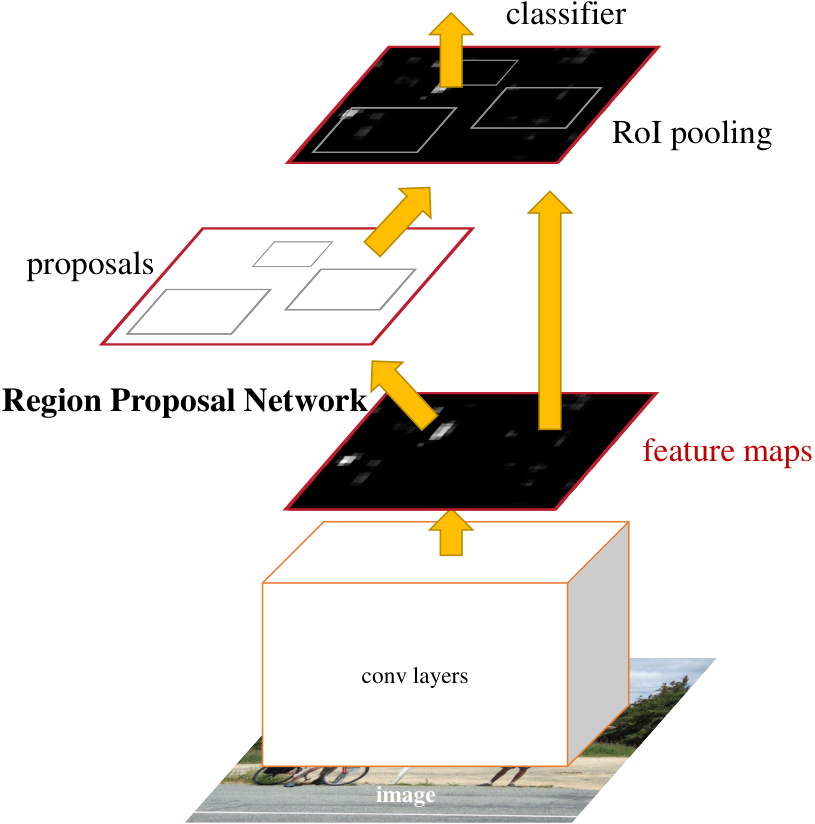
\includegraphics[width=0.68\textwidth]{figures/faster_rcnn_architecture_original.png}
\caption{Kiến trúc thống nhất của Faster R-CNN: RPN và bộ phát hiện dùng chung bản đồ đặc trưng. Hình được trích nguyên bản từ Ren và cộng sự, Hình 2 \cite{fasterrcnn}; không phải sơ đồ tự vẽ.}\label{fig:fasterrcnnarchitecture}
\end{figure}

Với ảnh ROD có xe ở xa và người ở gần, FPN cung cấp đặc trưng ở nhiều tỉ lệ còn RPN khoanh vùng ứng viên trước khi phân loại. Lợi thế tiềm tàng là quyết định theo vùng có thể phân tích chi tiết; đánh đổi là nhiều phép tính hơn. Cấu hình ứng dụng dùng head 26 đầu ra, gồm nền và 25 lớp ROD; nhãn nền không được hiển thị. 


\subsection{So sánh detector một giai đoạn và hai giai đoạn}
YOLO dự đoán trực tiếp trên ảnh; Faster R-CNN đề xuất vùng rồi phân tích region. Hai giai đoạn thêm overhead nhưng tập trung vào proposal; một giai đoạn gọn hơn nhưng vẫn có thể bỏ sót vật thể khó. Khác biệt framework/loss/transform khiến benchmark trên ROD cần thiết.

\paragraph{Diễn giải kiến trúc trong bối cảnh dự án.}
Số tham số chỉ là một đại lượng tài nguyên; latency còn phụ thuộc số phép toán, kích thước activation, cách xử lý proposal, kernel tối ưu và hậu xử lý. Một detector hai giai đoạn có thể chậm hơn trên CPU nhưng cho AP tốt hơn trên split cụ thể; điều đó không đồng nghĩa với hiệu quả tốt hơn trong mọi ngân sách. Ngược lại, model nhỏ có thể phù hợp về tốc độ nhưng vẫn cần kiểm tra lớp quan trọng và vật thể nhỏ. Vì vậy chương kết quả đặt metric và benchmark cạnh nhau thay vì đưa một thứ hạng tổng hợp duy nhất.

\section{Tăng cường dữ liệu và tối ưu huấn luyện}
Augmentation mô phỏng biến thiên không làm đổi nhãn: màu sắc, dịch chuyển, scale và lật ngang. Mosaic giúp mỗi ảnh đầu vào chứa nội dung từ nhiều ảnh nguồn, tăng ngữ cảnh và số object quan sát trong một batch. Lật dọc tắt vì cảnh đường phố lật ngược không thực tế; rotation và shear bằng 0 trong cấu hình hiện tại.

Augmentation quá mạnh có thể tạo cảnh không tự nhiên hoặc hộp rất nhỏ, còn quá yếu dễ overfit. Dự án không chạy ablation augmentation, nên không quy kết chênh lệch E3/E4 cho một phép biến đổi cụ thể. E6 code không có augmentation hình học tùy chỉnh ngoài transform chuẩn; đây là khác biệt giữa pipeline và là biến gây nhiễu khi so kiến trúc.
HSV jitter thay đổi sắc độ/màu, translate dịch ảnh, scale đổi kích thước, horizontal flip lật ngang, mosaic ghép nhiều ảnh. SGD tối ưu gradient minibatch; momentum làm trơn cập nhật; weight decay điều chuẩn; warmup tăng LR ban đầu; scheduler giảm LR theo thời gian. Không có ablation augmentation nên không quy kết cải thiện cho một phép biến đổi riêng.

Trong YOLO11, huấn luyện tối ưu đồng thời định vị hộp, phân loại và phân phối khoảng cách biên. Cấu hình E3/E4 đặt hệ số box 7,5; class 0,5 và DFL 1,5. Các hệ số xác định tỷ lệ đóng góp vào gradient, không phải mức quan trọng của lớp trong ứng dụng. Mosaic được bật, biến đổi HSV và lật ngang tạo thêm đa dạng; mixup, cutmix và copy-paste tắt. Hai run dùng cùng thiết lập nên khác biệt n/s được khảo sát trên nền tương đối đồng nhất.

Faster R-CNN trả các loss phân loại, hồi quy hộp, objectness RPN và hồi quy proposal. E6 chuyển nhãn YOLO chuẩn hóa thành hộp pixel \texttt{xyxy}, đặt \texttt{iscrowd=0}, và cộng một vào class ID vì Torchvision dành 0 cho background. Ảnh qua transform với cạnh ngắn 640, cạnh dài tối đa 960. Đây không phải resize vuông như YOLO, nên so sánh phản ánh pipeline hoàn chỉnh chứ không cô lập tuyệt đối kiến trúc.

Sau forward, hộp score thấp bị lọc và NMS loại dự đoán chồng lặp. NMS quá thấp có thể xóa hai vật thể gần nhau, quá cao có thể giữ nhiều hộp trùng. Evaluator thu prediction YOLO với NMS 0,7; Torchvision có hậu xử lý tích hợp. Đây là một nguyên nhân khiến metric log framework và evaluator chung không trùng hoàn toàn.
\section{Kết chương}
Metric, cách ghép, ngưỡng và hậu xử lý xác định ý nghĩa của so sánh. Kiến trúc tạo giả thuyết về đánh đổi; kết luận phải dựa trên checkpoint đã chấm cùng protocol. Chương tiếp theo mô tả dữ liệu, cấu hình và kết quả.
\chapter{XÂY DỰNG MÔ HÌNH HỌC MÁY}\label{chap:data}
\section{Thu thập dữ liệu}
Nguồn ROD gốc cung cấp ảnh và nhãn phát hiện vật cản trong cảnh đường phố \cite{rod}. Dự án sử dụng bản ROD Final A4 đã làm sạch và đóng băng; vì vậy các số liệu của bản Final không được đồng nhất với quy mô dataset card gốc.   Bảng~\ref{tab:split} nêu số lượng thực tế từ báo cáo freeze; không có ảnh TEST nào được dùng để lựa chọn ngưỡng, mô hình hay thông số huấn luyện trong bản thảo này.
Dữ liệu ROD được lưu dưới dạng ảnh cảnh đường phố cùng annotation detector. Bản sử dụng là Final A4 sau các bước kiểm tra, không đồng nhất số lượng với bản ROD công bố ban đầu.
\section{Phân tích và tiền xử lý dữ liệu}
\subsection{Thống kê dữ liệu}
\begin{table}[htbp]\centering
\caption{Quy mô ROD Final A4 theo split..}\label{tab:split}
\begin{tabular}{lrr}\toprule
Tập & Ảnh & Đối tượng được gán nhãn\\\midrule
TRAIN & 18.151 & 30.793\\
VALID & 3.318 & 5.320\\
TEST & 1.611 & 2.354\\\midrule
Tổng & 23.080 & 38.467\\\bottomrule
\end{tabular}
\end{table}
Tổng số liệu là 23.080 ảnh và 38.467 object; ảnh và object là hai đơn vị thống kê khác nhau. TRAIN dùng để học, VALID phục vụ lựa chọn, TEST giữ cho đánh giá cuối.
\subsection{Phân bố lớp và mất cân bằng}
ROD Final giữ thứ tự 25 lớp từ ID 0 đến 24: Bike, Building, Car, Person, Stairs, Traffic sign, Electrical Pole, Road, Motorcycle, Dustbin, Dog, Manhole, Tree, Guard rail, Pedestrian crosswalk, Truck, Bus, Bench, Traffic Cone, Fire hydrant, Teraffic Barrel, Plant Pot, Electrical Box, Chair và Bicycle Rack. Chuỗi ``Teraffic Barrel'' được giữ đúng theo \texttt{data.yaml}. Nếu chỉ sửa tên ở một nơi, checkpoint và giao diện vẫn chạy nhưng nhãn hiển thị có thể lệch với evaluator; taxonomy vì vậy là một phần của hợp đồng dữ liệu.

Các lớp bao phủ ba nhóm chính. Nhóm tác nhân chuyển động gồm người, xe đạp, xe máy, ô tô, xe buýt, xe tải và chó. Nhóm cấu trúc đường đi gồm Road, Stairs, Manhole, Guard rail và Pedestrian crosswalk. Nhóm vật thể ven đường gồm biển báo, cột điện, thùng rác, ghế, chậu cây, hộp điện, cọc tiêu, thùng chắn và giá xe đạp. Phân nhóm chỉ hỗ trợ thảo luận; model vẫn học 25 lớp độc lập và không có nhãn cấp cha.

Phân bố lớp không cân bằng. mAP cho mỗi lớp trọng số bằng nhau, trong khi micro Precision/Recall bị chi phối nhiều hơn bởi lớp có nhiều object. Một mô hình có micro Recall cao vẫn có thể bỏ sót lớp hiếm; ngược lại mAP cao không cho biết số cảnh báo sai thực tế tại ngưỡng vận hành. Vì thế báo cáo đọc đồng thời chỉ số tổng, TP/FP/FN và AP theo lớp.

\begin{figure}[H]\centering
\IfFileExists{../../results/lam_sach_du_lieu/analysis/fig_class_distribution.png}
  {\includegraphics[width=0.88\textwidth]{../../results/lam_sach_du_lieu/analysis/fig_class_distribution.png}}
  {\fbox{\parbox[c][5cm][c]{0.82\textwidth}{\centering Biểu đồ phân bố lớp\\(không có tệp ảnh trong workspace biên dịch)}}}
\caption{Phân bố đối tượng theo lớp ở lần phân tích dữ liệu nguồn; số liệu Final lấy từ báo cáo đóng băng.}\label{fig:classdist}
\end{figure}
\subsection{Kiểm tra ảnh và nhãn}
Nhãn được mã hóa bằng chỉ số lớp và hộp bao theo hệ tọa độ YOLO. Vấn đề khi dùng chung hai framework là Torchvision dành chỉ số không cho nền, còn bộ ROD đánh số lớp từ không. Bộ chuyển đổi suy luận ánh xạ nhãn foreground Torchvision sang ROD bằng cách trừ một và bỏ nền, nhờ đó các kết quả đánh giá có chung lớp.  Ví dụ, Bike và Motorcycle là hai lớp khác nhau trong bảng nhãn, nên việc phát hiện đúng vị trí nhưng nhầm giữa chúng vẫn là lỗi phân loại. Đây cũng là lý do không thể suy luận chất lượng chỉ từ hình minh họa có hộp bao.
Kiểm tra cú pháp và hình học hộp không chứng minh annotation đúng về ngữ nghĩa. Còn 18 đề xuất bbox và các trường hợp nhầm Bike/Motorcycle chưa giải quyết triệt để; không xem toàn bộ đề xuất relabel là đã hoàn tất.
\subsection{Kiểm tra rò rỉ giữa các split}
Báo cáo freeze ghi nhận không còn trùng nội dung ảnh chính xác giữa các split và không có lỗi cú pháp hay hình học hộp bao; nó vẫn ghi nhận nhóm trùng trong cùng split và một số nhãn còn chờ duyệt.  Kiểm tra trùng chính xác không chứng minh mọi ảnh gần trùng đều đã được loại, còn kiểm tra nhãn hợp lệ không chứng minh nhãn đúng về ngữ nghĩa. Do đó, chất lượng đánh giá có giới hạn từ dữ liệu và chưa nên diễn giải một sai khác nhỏ giữa mô hình như tác động chắc chắn ngoài tập VALID.
Sau freeze không còn exact duplicate xuyên split, nhưng còn 271 nhóm exact duplicate trong cùng split. Exact hash không nhận diện mọi near-duplicate do crop, resize hoặc nén lại.
\subsection{Chuỗi làm sạch V2, V3, V4 và Final A4}
Bản nguồn có 24.326 ảnh và 40.195 object. V2 còn 24.187 ảnh và 40.041 object sau khi loại 139 cặp ảnh--nhãn cùng bốn annotation sai được xác nhận. V3 giữ nguyên quy mô và áp dụng bảy relabel Bike sang Motorcycle đã được duyệt; 152 đề xuất khác và 18 đề xuất bbox còn chờ xử lý. V4 cách ly 929 cặp có cạnh leakage trực tiếp, đưa dữ liệu về 23.258 ảnh và 38.797 object. Final cách ly thêm 178 ảnh, gồm 146 TRAIN và 32 VALID, không thay đổi TEST.

\begin{table}[H]\centering
\caption{Thay đổi quy mô dữ liệu qua các mốc làm sạch}\label{tab:cleaning}
\begin{tabular}{lrrp{6.1cm}}\toprule
Mốc & Ảnh & Object & Thay đổi chính\\\midrule
Nguồn & 24.326 & 40.195 & Chuyển đổi nhãn và kiểm toán độc lập.\\
V2 & 24.187 & 40.041 & Loại 139 cặp và annotation sai đã xác nhận.\\
V3 & 24.187 & 40.041 & Relabel 7 trường hợp Bike sang Motorcycle.\\
V4 & 23.258 & 38.797 & Cách ly 929 cặp có leakage trực tiếp.\\
Final A4 & 23.080 & 38.467 & Cách ly thêm 178 ảnh, giữ nguyên TEST.\\\bottomrule
\end{tabular}
\end{table}

Final cách ly thêm 178 ảnh theo manifest; 146 ảnh thuộc TRAIN, 32 thuộc VALID và 0 thuộc TEST. Báo cáo xác nhận 0 ảnh thiếu label, 0 label thiếu ảnh, 0 lỗi class ID/cú pháp/hình học và 0 nhóm exact duplicate xuyên split. Tuy vậy còn 271 nhóm exact duplicate trong cùng split, 18 đề xuất bbox và các relabel Bike/Motorcycle chưa duyệt. Chúng là giới hạn dữ liệu, không phải lỗi đã xử lý.
Các con số đóng băng còn cho phép phân biệt quy mô annotation với số ảnh. Khi lớp xuất hiện không đều, cùng một Recall tổng có thể che khuất thiếu hụt ở một lớp hiếm. Bảng AP theo lớp ở phần kết quả vì vậy là phần bổ sung cho thống kê tổng, còn phân tích định tính vẫn cần được thực hiện trên các prediction cụ thể. Không ngoại suy tần suất từ số object trong VALID sang mọi môi trường sử dụng.

\subsection{Đóng băng TRAIN, VALID và TEST}
TRAIN dùng cập nhật trọng số. VALID dùng theo dõi checkpoint, chọn ngưỡng và so sánh mô hình. TEST chỉ ước lượng cuối sau khi mọi quyết định đã khóa. Nếu ngưỡng được hạ vì một ảnh TEST khó, ảnh đó không còn độc lập và kết quả sẽ lạc quan. Bởi vậy script TEST kiểm hash dữ liệu, checkpoint, ngưỡng và protocol trước khi chạy.

Exact hash phát hiện bản sao byte giống hệt, còn manifest xử lý các quan hệ leakage đã xác định. Nó không chứng minh đã loại mọi near-duplicate do crop, resize hoặc nén lại. Kiểm toán tiếp theo có thể dùng embedding hay perceptual hash với duyệt thủ công; không nên tự động loại ảnh chỉ vì khoảng cách gần nếu chưa xác nhận cùng cảnh.


TEST không được dùng để lựa chọn mô hình, threshold hoặc preprocessing. Sau khi khóa các quyết định bằng VALID, ba mô hình đã được đánh giá đúng một lượt trên TEST; kết quả cuối được trình bày tại Bảng~\ref{tab:testsummary}.
\section{Xây dựng mô hình học máy}
\subsection{Tạo Dataset và DataLoader}
YOLO đọc ảnh và nhãn class ID, tâm, rộng, cao chuẩn hóa; E3/E4 dùng batch 8 và input 640. E6 dùng Dataset trả ảnh cùng box pixel xyxy và nhãn foreground, batch 2. Validation giữ thứ tự cố định, không sử dụng augmentation ngẫu nhiên. Trước train cần kiểm tra class range, box rỗng, dtype, shape và cặp ảnh-nhãn để tránh lỗi dữ liệu bị nhầm với lỗi mô hình.
\subsection{Ánh xạ nhãn giữa YOLO và Torchvision}
ROD/YOLO dùng class ID 0--24. Torchvision dành ID 0 cho background, do đó target foreground ánh xạ sang 1--25; đầu ra inference bỏ 0 rồi trừ một. Danh sách ánh xạ đầy đủ đặt ở phụ lục. Tên lớp “Teraffic Barrel” được giữ nguyên theo data.yaml.
\subsection{Cấu hình E3 YOLO11n}
E3 dùng COCO pretrained, imgsz 640, batch 8, SGD, lr0 0,01, lrf 0,01, momentum 0,937, weight decay 0,0005, \texttt{warmup\_epochs}=3, seed 0; box 7,5, cls 0,5, dfl 1,5; mosaic 1,0, scale 0,5, fliplr 0,5.
\subsection{Cấu hình E4 YOLO11s}
E4 dùng YOLO11s COCO pretrained và cùng cấu hình chính như E3. Cả hai run dừng sau 10 epoch đầu của lịch LR cấu hình cho 30 epoch; đây không phải lịch 10 epoch được thiết kế lại. Pha close-mosaic ở 10 epoch cuối chưa xảy ra.
\subsection{Cấu hình E6 Faster R-CNN}
E6 dùng Faster R-CNN ResNet-50 FPN V2 COCO V2 pretrained, predictor 26 đầu ra, 10 epoch, batch 2, SGD, LR 0,005, momentum 0,9, weight decay 0,0005, StepLR(\texttt{step\_size}=3, gamma=0,1), \texttt{min\_size}=640 và \texttt{max\_size}=960. Log huấn luyện rời của E6 thiếu tại local nên không dựng learning curve, GPU hay thời gian huấn luyện.
\begin{table}[H]\centering\small
\caption{Cấu hình fine-tune ba mô hình}\label{tab:traincfg}
\begin{tabular}{p{2.8cm}p{3.2cm}p{3.2cm}p{4.2cm}}\toprule
Thuộc tính & E3 & E4 & E6\\\midrule
Khởi tạo & COCO & COCO & COCO V2\\
Epoch & 10/30 lịch LR & 10/30 lịch LR & 10\\
Input & 640 & 640 & min 640; max 960\\
Batch & 8 & 8 & 2\\
Optimizer & SGD & SGD & SGD\\
LR/scheduler & 0,01; lrf 0,01; warmup 3 & như E3 & 0,005; StepLR(3; 0,1)\\
Momentum/decay & 0,937/0,0005 & 0,937/0,0005 & 0,9/0,0005\\
Seed & 0 & 0 & theo cấu hình còn lưu\\
Loss/augment & box 7,5; cls 0,5; dfl 1,5; mosaic 1,0; scale 0,5; flip 0,5 & như E3 & predictor 26 lớp\\
\bottomrule\end{tabular}\end{table}
Sự khác nhau giữa optimizer và kiến trúc cũng ảnh hưởng độ hội tụ. Weight decay và momentum không có tác động độc lập với learning rate; cùng một giá trị có thể cho diễn tiến khác khi batch size hoặc số bước cập nhật đổi. E3/E4 có batch lớn hơn E6, input transform YOLO khác transform Torchvision, và scheduler cũng không đồng nhất. Không thể chỉ nhìn bảng hyperparameter để kết luận mọi mô hình nhận ngân sách tối ưu tương đương; bảng này mô tả các cấu hình được khai báo và các giới hạn log hiện có.

\subsection{Cơ chế checkpoint và resume}
Ba checkpoint có SHA256 đã khóa: E3 \texttt{41f794...ed02}, E4 \texttt{dc09c7...e2f5}, E6 \texttt{ce459c...f9bd}. Adapter từ chối chạy khi hash sai. E6 mang đuôi \texttt{.zip} nhưng là state dictionary PyTorch, không phải archive; model được dựng lại bằng builder V2 với head 26 lớp và nạp strict.

Best checkpoint E3 có 5.477.402 byte, E4 19.191.770 byte, E6 173.898.073 byte. Kích thước tệp không bằng bộ nhớ runtime vì activation và workspace phụ thuộc ảnh, framework và thiết bị. Nó vẫn phản ánh chi phí lưu trữ và góp phần vào thời gian request đầu khi model chưa cache.
\subsection{Tiêu chí chọn best checkpoint}
YOLO dùng fitness nội bộ có liên hệ mAP50--95; E6 dùng tiêu chí VALID trong pipeline riêng. Vì framework khác nhau, các metric huấn luyện không được đặt làm bảng xếp hạng chung. Ba checkpoint best được chấm lại bằng evaluator chung.
\subsection{Giao thức chọn confidence threshold}
Threshold được tìm từ prediction VALID đã cache, quét theo micro-F2 với quy tắc tie-break cố định. Giá trị E3/E4/E6 là 0,22/0,19/0,59. Confidence score không được hiệu chuẩn xác suất; threshold không thay đổi theo TEST.
\subsection{Giao thức đánh giá chung}
Ground truth YOLO được chuyển từ tâm--rộng--cao chuẩn hóa sang hai góc pixel. Prediction E6 đổi foreground 1--25 về ROD 0--24; background bị bỏ. AP dùng 101 điểm recall tại IoU 0,50 đến 0,95, bước 0,05 và tối đa 100 detection/ảnh. Precision/Recall vận hành ghép tại IoU 0,50 với tối đa 300 detection/ảnh.

ROD không có nhãn crowd/ignore nên evaluator đặt area=all và không bỏ qua crowd. “COCO-style” chỉ mô tả dải IoU và nội suy; implementation không phải pycocotools chính thức. Ba JSON kết quả lưu protocol bên cạnh metric để số đo không bị tách khỏi định nghĩa.
Evaluator dùng phong cách COCO cho dải IoU và nội suy nhưng là implementation riêng, không phải pycocotools chính thức. Ngưỡng vận hành và prediction cache được ghi riêng để không trộn metric framework với metric chung.
\subsection{Khóa TEST và nguyên tắc lựa chọn}
Sau VALID, \texttt{evaluation\_lock.json} ghi hash data YAML, confidence config, checkpoint và protocol. Script TEST yêu cầu khóa hợp lệ cùng cờ xác nhận. Nếu model, threshold hoặc protocol đổi sau khi xem TEST, kết quả không còn độc lập và phải được coi là thí nghiệm khác.

TEST đã chạy đúng một lượt trên 1.611 ảnh sau khi khóa checkpoint, ngưỡng và evaluator. Kết quả trạng thái \texttt{FINAL\_LOCKED} được báo theo metric tổng và theo 25 lớp; không có quyết định nào được điều chỉnh từ TEST.
\section{Phân tích kết quả thực nghiệm}\label{chap:results}
\subsection{Kết quả E3 YOLO11n}
Ở threshold 0,22, E3 đạt Precision 0,6455, Recall 0,7733 và F2 0,7439. Đây là kết quả VALID tại epoch 10, tức 10 epoch đầu của lịch 30 epoch; kết quả này không chứng minh mô hình đã hội tụ.
\subsection{Kết quả E4 YOLO11s}
Ở threshold 0,19, E4 đạt Precision 0,6502, Recall 0,8075 và F2 0,7703. Mô hình phát hiện thêm 182 ground truth so với E3, đồng thời phát sinh thêm 52 FP; chênh lệch cần được xác nhận trên TEST độc lập.
\subsection{Kết quả E6 Faster R-CNN}
Ở threshold 0,59, E6 đạt Precision 0,7483, Recall 0,8453 và F2 0,8239. Đây là kết quả VALID; checkpoint cho phép đánh giá nhưng không thay thế log huấn luyện E6 còn thiếu.
\subsection{So sánh Precision và Recall}
Bảng~\ref{tab:fullmetrics} tập hợp Precision, Recall và F2 từ cùng evaluator; threshold riêng được chọn trên VALID. Các bảng tiếp theo tách chất lượng xếp hạng và số đếm vận hành để giữ bố cục dễ đọc.
\begin{table}[H]\centering\small
\caption{Precision, Recall và F2 trên VALID}\label{tab:fullmetrics}
\begin{tabular}{lrrrr}\toprule
Mô hình & Threshold & Precision & Recall & F2\\\midrule
E3 & 0,22 & 0,6455358544 & 0,7733082707 & 0,7438614255\\
E4 & 0,19 & 0,6502194642 & 0,8075187970 & 0,7702513716\\
E6 & 0,59 & 0,7482529118 & 0,8453007519 & 0,8239281788\\
\bottomrule\end{tabular}\end{table}
Ở ngưỡng vận hành đã chọn, E6 có cả Precision và Recall cao nhất trên VALID; E4 cải thiện Recall so với E3 với mức tăng Precision nhỏ. Vì ngưỡng được tối ưu trên chính VALID, các số này mô tả lựa chọn vận hành trên tập xác thực chứ không phải ước lượng độc lập cuối cùng.

\subsection{So sánh mAP50 và mAP50--95}
E4 tăng mAP50--95 khoảng 0,0194 so với E3; E6 cao hơn cả hai. mAP50 đo mức ghép dễ hơn, còn trung bình đến IoU 0,95 nhạy với chất lượng định vị. Mức giảm theo IoU thể hiện yêu cầu hộp chặt hơn chứ không xác định riêng nguyên nhân của lỗi.
\begin{table}[H]\centering\small
\caption{mAP trên VALID theo evaluator chung}\label{tab:mapvalid}
\begin{tabular}{lrr}\toprule
Mô hình & mAP50 & mAP50--95\\\midrule
E3 & 0,7957589188 & 0,5951288215\\
E4 & 0,8048659705 & 0,6145455259\\
E6 & 0,8701219838 & 0,6604099804\\
\bottomrule\end{tabular}\end{table}
Thứ hạng mAP nhất quán với các chỉ số vận hành tổng thể, nhưng mAP tổng hợp không cho biết lớp nào gây ra chênh lệch. Vì vậy cần đọc bảng theo lớp cùng phân tích lỗi; mức cải thiện trên VALID vẫn phải được kiểm tra trên TEST theo giao thức đã khóa.

\subsection{Phân tích TP, FP và FN}
Tại ngưỡng vận hành, E3 có 4.114 TP, 2.259 FP và 1.206 FN; E4 có 4.296 TP, 2.311 FP và 1.024 FN; E6 có 4.497 TP, 1.513 FP và 823 FN. E4 tìm thêm 182 GT so với E3 nhưng phát sinh thêm 52 FP. E6 vừa giảm FN 201 vừa giảm FP 798 so với E4 trên VALID. Vì threshold được chọn bằng F2 trên cùng tập, lợi ích này phải được xác nhận trên TEST.

\begin{table}[H]\centering\small
\caption{Số lượng TP, FP và FN trên VALID}\label{tab:countsvalid}
\begin{tabular}{lrrr}\toprule
Mô hình & TP & FP & FN\\\midrule
E3 & 4.114 & 2.259 & 1.206\\
E4 & 4.296 & 2.311 & 1.024\\
E6 & 4.497 & 1.513 & 823\\
\bottomrule\end{tabular}\end{table}
Ở các ngưỡng tương ứng, E4 phát hiện thêm 182 đối tượng so với E3 và có thêm 52 dự đoán dương tính sai; E6 giảm đồng thời FP và FN so với E4 trên VALID. Đây là số đếm gộp, nên chưa phản ánh độ nghiêm trọng, kích thước hay bối cảnh của từng lỗi.
Các giá trị nhiều chữ số thập phân trong các bảng phục vụ đối chiếu tệp kết quả, không hàm ý độ bất định thống kê thấp. Mỗi metric VALID được ước lượng trên một tập hữu hạn và một checkpoint; khi diễn giải nên tập trung vào quy mô chênh lệch cùng giới hạn thiết kế, thay vì coi các chữ số cuối là bằng chứng về ưu thế chắc chắn.

\begin{figure}[H]\centering
\IfFileExists{../../results/E3_YOLO11n/metrics/plots/results.png}
  {\includegraphics[width=0.82\textwidth]{../../results/E3_YOLO11n/metrics/plots/results.png}}
  {\fbox{\parbox[c][5cm][c]{0.78\textwidth}{\centering Đường cong huấn luyện E3\\(không có tệp ảnh trong workspace biên dịch)}}}
\caption{Đường cong huấn luyện E3 YOLO11n trong 10 epoch đầu của lịch 30 epoch.}\label{fig:e3curve}
\end{figure}

Log E3 epoch 10 ghi Precision 0,84610, Recall 0,73533 và mAP50--95 0,60605. Số khác bảng evaluator chung vì threshold, NMS, max detection và tích phân AP khác nhau. Báo cáo không trộn hai protocol trong một bảng xếp hạng; log chỉ dùng đọc xu hướng huấn luyện.
\clearpage
\subsection{Phân tích kết quả theo 25 lớp}
\begin{table}[H]\centering\small
\caption{AP50--95 theo lớp trên VALID}\label{tab:perclass}
\begin{tabular}{lrrr}
\toprule Lớp & E3 & E4 & E6\\\midrule
Bike & 0,618 & 0,650 & 0,782\\ Building & 0,652 & 0,646 & 0,635\\
Car & 0,571 & 0,593 & 0,619\\ Person & 0,445 & 0,473 & 0,539\\
Stairs & 0,529 & 0,582 & 0,614\\ Traffic sign & 0,293 & 0,364 & 0,380\\
Electrical Pole & 0,451 & 0,433 & 0,503\\ Road & 0,407 & 0,434 & 0,513\\
Motorcycle & 0,459 & 0,457 & 0,439\\ Dustbin & 0,752 & 0,758 & 0,769\\
Dog & 0,677 & 0,747 & 0,768\\ Manhole & 0,772 & 0,808 & 0,803\\
Tree & 0,517 & 0,490 & 0,549\\ Guard rail & 0,410 & 0,373 & 0,520\\
Pedestrian crosswalk & 0,314 & 0,345 & 0,502\\ Truck & 0,567 & 0,578 & 0,657\\
Bus & 0,593 & 0,627 & 0,658\\ Bench & 0,624 & 0,697 & 0,710\\
Traffic Cone & 0,634 & 0,647 & 0,643\\ Fire hydrant & 0,863 & 0,906 & 0,847\\
Teraffic Barrel & 0,849 & 0,844 & 0,896\\ Plant Pot & 0,702 & 0,720 & 0,743\\
Electrical Box & 0,868 & 0,884 & 0,931\\ Chair & 0,671 & 0,715 & 0,715\\
Bicycle Rack & 0,640 & 0,592 & 0,775\\
\bottomrule
\end{tabular}
\end{table}

Traffic sign thấp nhất ở cả ba model, còn Electrical Box, Teraffic Barrel và Fire hydrant thuộc nhóm cao. Person và Pedestrian crosswalk quan trọng trong cảnh di chuyển nhưng AP thấp hơn nhiều lớp cố định. E6 cải thiện mạnh Pedestrian crosswalk và Bicycle Rack so với E4, nhưng Motorcycle giảm. mAP tổng cao hơn không đồng nghĩa tốt hơn ở mọi lớp.

Số GT theo lớp khác nhau, nên AP của lớp hiếm có độ bất định lớn. Báo cáo chưa bootstrap khoảng tin cậy và chưa lặp theo seed. Chênh lệch rất nhỏ, như Manhole giữa E4 và E6, không nên diễn giải thành ưu thế chắc chắn. Bảng lớp dùng để ưu tiên kiểm tra ảnh lỗi và thiết kế dữ liệu bổ sung.
\clearpage
\section{Kết quả đánh giá cuối trên tập TEST}
Tập TEST gồm 1.611 ảnh và 2.354 đối tượng ground truth. Ba checkpoint được đánh giá sau khi \texttt{evaluation\_lock.json} đã khóa checkpoint, ngưỡng confidence, ánh xạ lớp và giao thức. Các ngưỡng 0,22/0,19/0,59 lần lượt của E3/E4/E6 được chọn từ VALID và không điều chỉnh sau khi xem TEST. Cả ba kết quả có trạng thái \texttt{FINAL\_LOCKED} trong \texttt{results/final\_test\_summary.json}.

\begin{table}[H]\centering\small
\caption{Kết quả tổng hợp cuối trên TEST theo evaluator chung}\label{tab:testsummary}
\begin{tabular}{lrrrrrrrr}\toprule
Mô hình & Ngưỡng & Precision & Recall & F2 & mAP50 & mAP50--95 & TP/FP/FN\\\midrule
E3 YOLO11n & 0,22 & 0,6551 & 0,7392 & 0,7207 & 0,7518 & 0,5548 & 1740/916/614\\
E4 YOLO11s & 0,19 & 0,6662 & 0,7732 & 0,7491 & 0,7774 & 0,5807 & 1820/912/534\\
E6 Faster R-CNN & 0,59 & 0,7570 & 0,8496 & 0,8293 & 0,8754 & 0,6782 & 2000/642/354\\
\bottomrule\end{tabular}\end{table}

Trên TEST độc lập, E4 tăng Recall 0,0340 và mAP50--95 0,0259 so với E3, đồng thời Precision tăng 0,0111. E6 đạt các chỉ số tổng hợp cao nhất: so với E4, Recall tăng 0,0765, Precision tăng 0,0908 và mAP50--95 tăng 0,0975; số FN giảm từ 534 xuống 354 và FP giảm từ 912 xuống 642. Kết quả này chỉ áp dụng cho checkpoint, split và evaluator đã khóa; một lần chạy TEST không ước lượng được biến thiên do seed.

\begin{longtable}{lrrrr}
\caption{AP50--95 theo 25 lớp trên TEST}\label{tab:testperclass}\\
\toprule Lớp & Số GT & E3 & E4 & E6\\\midrule
\endfirsthead
\toprule Lớp & Số GT & E3 & E4 & E6\\\midrule
\endhead
Bike & 48 & 0,652 & 0,690 & 0,803\\
Building & 54 & 0,645 & 0,707 & 0,739\\
Car & 247 & 0,534 & 0,540 & 0,610\\
Person & 320 & 0,398 & 0,411 & 0,574\\
Stairs & 222 & 0,522 & 0,557 & 0,596\\
Traffic sign & 104 & 0,410 & 0,392 & 0,527\\
Electrical Pole & 42 & 0,473 & 0,500 & 0,629\\
Road & 37 & 0,432 & 0,418 & 0,518\\
Motorcycle & 38 & 0,439 & 0,451 & 0,505\\
Dustbin & 45 & 0,362 & 0,448 & 0,511\\
Dog & 30 & 0,594 & 0,396 & 0,773\\
Manhole & 242 & 0,790 & 0,813 & 0,830\\
Tree & 150 & 0,510 & 0,457 & 0,581\\
Guard rail & 69 & 0,389 & 0,379 & 0,634\\
Pedestrian crosswalk & 189 & 0,461 & 0,490 & 0,588\\
Truck & 43 & 0,513 & 0,543 & 0,646\\
Bus & 55 & 0,527 & 0,573 & 0,614\\
Bench & 28 & 0,656 & 0,769 & 0,776\\
Traffic Cone & 92 & 0,586 & 0,627 & 0,674\\
Fire hydrant & 25 & 0,854 & 0,895 & 0,888\\
Teraffic Barrel & 19 & 0,859 & 0,838 & 0,977\\
Plant Pot & 34 & 0,614 & 0,620 & 0,721\\
Electrical Box & 34 & 0,557 & 0,714 & 0,842\\
Chair & 151 & 0,656 & 0,693 & 0,704\\
Bicycle Rack & 36 & 0,437 & 0,597 & 0,694\\
\bottomrule
\end{longtable}

E6 đạt AP50--95 cao nhất ở 24/25 lớp; ngoại lệ là Fire hydrant, nơi E4 đạt 0,8952 so với 0,8877 của E6. Các lớp khó nhất của cả ba mô hình tập trung ở nhóm có hình dạng, bối cảnh hoặc nhãn dễ biến thiên như Person, Traffic sign, Road và Motorcycle. Teraffic Barrel có AP cao nhưng chỉ có 19 ground truth, vì vậy không nên diễn giải chênh lệch nhỏ ở lớp hiếm như bằng chứng tổng quát. TEST chỉ dùng để báo cáo cuối; không có ngưỡng hay checkpoint nào được chọn lại từ các số liệu này.
\subsection{So sánh độ trễ và tài nguyên}
Độ trễ được đo trên cùng 30 ảnh VALID, một ảnh mỗi lượt, sau các lượt làm nóng. Mức FPS ở đây là nghịch đảo thời gian suy luận trung bình khi xử lý tuần tự, không phải tốc độ webcam hay toàn hệ thống.  Bảng~\ref{tab:benchfull} cho thấy E4 dùng nhiều tham số và chậm hơn E3; E6 nặng hơn rõ rệt trên CPU đã đo.



Theo cùng benchmark, E4 có độ trễ trung bình gấp 2,44 lần và số tham số gấp 3,64 lần E3.  Lợi ích Recall của E4 vì vậy có chi phí cụ thể; lựa chọn phụ thuộc yêu cầu vận hành hơn là một bảng xếp hạng đơn. E6 đạt Recall VALID cao nhất, nhưng độ trễ trung bình CPU gấp 13,51 lần E4.  Kết quả này chỉ áp dụng cho CPU và phương pháp đo đã ghi, không dự đoán tốc độ GPU hay thiết bị di động.

Benchmark callback tính thêm xác thực ảnh, vẽ hộp, lưu PNG và tổng hợp văn bản. Thời gian trung bình sau warmup lần lượt là 134,13 ms cho E3, 232,63 ms cho E4 và 2.535,22 ms cho E6; request đầu dài hơn do tải model và thiết lập.  Callback vẫn chưa bao gồm thời gian tải ảnh qua mạng, dựng giao diện trình duyệt hay tương tác con người. Do đó, câu hỏi ``có real-time hay không'' hiện CHƯA ĐO cần định nghĩa mục tiêu độ trễ, đo end-to-end trên phần cứng triển khai và với luồng video nếu phạm vi sản phẩm thay đổi. Chỉ số VRAM cũng chưa đo được trong benchmark CPU. 



\begin{table}[H]\centering\small
\caption{Benchmark CPU trên 30 ảnh VALID, batch 1}\label{tab:benchfull}
\begin{tabular}{lrrrr}\toprule
Mô hình & Tham số & Mean (ms) & p95 (ms) & FPS\\\midrule
E3 & 2.594.715 & 76,26 & 87,52 & 13,11\\
E4 & 9.437.467 & 185,83 & 360,94 & 5,38\\
E6 & 43.379.153 & 2.511,30 & 3.040,27 & 0,40\\
\bottomrule\end{tabular}\end{table}


Request đầu E4 thấp hơn E3 trong mẫu không có nghĩa E4 luôn tải nhanh hơn; cache hệ điều hành và thứ tự chạy có thể ảnh hưởng. Mean/p95 sau warmup phù hợp hơn để mô tả vận hành lặp lại. Callback gần inference ở E6 vì forward chiếm phần lớn thời gian, còn E3/E4 cho thấy chi phí vẽ và lưu ảnh.

Ngưỡng tự động là 0,22, 0,19 và 0,59; VALID là 0,7439, 0,7703 và 0,8239. Không có slider giúp kết quả nhất quán, nhưng một ngưỡng cho mỗi model không tối ưu riêng từng lớp. Per-class threshold mới chỉ được khám phá và chưa áp dụng để tránh tăng độ phức tạp khi chưa đánh giá ổn định.
\begin{table}[H]\centering\small
\caption{Độ trễ callback CPU trên 30 ảnh VALID}\label{tab:callback}
\begin{tabular}{lrrr}\toprule
Model & Request đầu (ms) & Mean warm (ms) & p95 (ms)\\\midrule
E3 & 975,35 & 134,13 & 209,83\\
E4 & 653,88 & 232,63 & 301,20\\
E6 & 5.061,34 & 2.535,22 & 2.692,17\\
\bottomrule\end{tabular}\end{table}
\subsection{Hạn chế của thực nghiệm}
Các threshold được chọn trên VALID; không có nhiều seed hay bootstrap khoảng tin cậy. E3/E4 mới chạy mười epoch đầu của lịch 30 epoch, log huấn luyện E6 thiếu. Dữ liệu còn 271 nhóm trùng trong split và vấn đề nhãn. TEST đã được đo theo cấu hình khóa; VRAM/GPU, điện năng, thời gian trên máy đích và thử nghiệm người dùng vẫn CHƯA ĐO.

Các kết quả cần được đọc trong bối cảnh quy trình chọn mô hình. Checkpoint và ngưỡng confidence dựa trên VALID nên có thể thích nghi với đặc điểm tập xác thực. TEST đã được giữ độc lập và chỉ mở sau khi checkpoint, mapping lớp, quy tắc NMS và evaluator được khóa; vì vậy Bảng~\ref{tab:testsummary} là phép đo cuối, còn VALID tiếp tục được giữ để giải thích quá trình lựa chọn.

Benchmark hiện phản ánh một môi trường CPU, batch 1 và 30 ảnh; mẫu nhỏ này có ích cho so sánh tương đối trong cùng máy nhưng không đại diện toàn bộ phân bố tải thực tế. Kết quả còn phụ thuộc trạng thái cache, số luồng, phiên bản thư viện, thao tác tiền xử lý và hậu xử lý. Đặc biệt, trung bình latency không cho thấy các trường hợp đuôi dài khi ảnh phức tạp hoặc số proposal tăng. Một đánh giá triển khai tiếp theo nên lưu môi trường phần mềm, lặp nhiều lượt, báo median và p95 cùng độ phân tán; nếu nhắm thiết bị di động cần đo trực tiếp trên chính thiết bị thay vì ngoại suy từ CPU phát triển.

Cuối cùng, bộ dữ liệu cân bằng hay đầy đủ không thể chỉ được suy ra từ tổng số ảnh. Các lớp có ít mẫu và những nhóm nhãn gần nghĩa có thể có sai số lớn hơn, trong khi duplicate cùng split làm giảm số cảnh độc lập hiệu dụng. Do đó, bảng phân lớp nên được nối với xem xét ảnh FN/FP có lấy mẫu theo quy tắc và được kiểm tra thủ công. Việc xem lỗi chỉ có vai trò mô tả hoặc định hướng nghiên cứu tiếp theo; không được dùng để sửa kết quả TEST sau khi đã quan sát dự đoán.
\section{Kết chương}
E6 có metric VALID cao nhất nhưng latency CPU lớn nhất; E3 nhanh nhất; E4 ở giữa với Recall cao hơn E3. Không có model nào được xác nhận là phù hợp cho mọi thiết bị hoặc an toàn trong thực tế.
\chapter{XÂY DỰNG ỨNG DỤNG PHÁT HIỆN VẬT CẢN}\label{chap:app}
\section{Triển khai các chức năng nghiệp vụ}
\subsection{Kiến trúc ứng dụng}
Gradio nhận JPG/JPEG/PNG, cho chọn E3/E4/E6, chạy adapter, vẽ bbox và trả PNG cùng danh sách detection. Adapter chuẩn hóa class ID, tọa độ, score và thời gian. Model được cache tối đa ba instance; CUDA được chọn khi có, nếu không dùng CPU. Đường dẫn checkpoint cố định và hash được kiểm trước khi load.

Thời gian suy luận đo riêng quanh model. Thời gian callback bắt đầu từ đối tượng PIL và kết thúc sau kiểm ảnh, inference, vẽ, lưu PNG và tạo văn bản. Nó không gồm upload qua mạng, hàng đợi server và browser render. Tách hai phạm vi đo giúp tránh gọi inference latency là trải nghiệm end-to-end.


\subsection{Tải ảnh đầu vào}
Ứng dụng nhận JPG/JPEG/PNG tải lên, kiểm tra ảnh giải mã được rồi chuyển sang adapter. Ảnh lỗi cần được xử lý thành thông báo, không làm sập callback. Chức năng hiện tại là ảnh đơn, không có camera.
\subsection{Chọn mô hình}
Người dùng chọn E3, E4 hoặc E6; adapter dùng checkpoint, preprocessing và mapping tương ứng. Cache model tránh khởi tạo lại mỗi lần. CUDA sử dụng khi có; nếu không thì CPU fallback. Khả năng chạy trên CPU không đồng nghĩa đạt latency phù hợp realtime.
\subsection{Auto Confidence}
Ngưỡng tự động E3/E4/E6 lần lượt 0,22/0,19/0,59, được chốt bằng VALID. Score khác kiến trúc không cùng thang xác suất; không có ngưỡng nào được chọn từ TEST.
\paragraph{Vòng đời một yêu cầu.}
Sau khi người dùng tải ảnh, callback xác thực dữ liệu, lấy adapter theo model, áp dụng threshold, chuẩn hóa tọa độ/lớp, vẽ overlay, mã hóa PNG và tạo phần thống kê. Tách các bước cho phép kiểm thử đơn vị theo từng hợp đồng. Cache giảm cold-start ở request tiếp theo nhưng giữ model trong bộ nhớ; điều này cần được xem xét nếu máy chủ có ít RAM hoặc nhiều người dùng đồng thời. Benchmark hiện tại không đo concurrency hay áp lực tải nhiều request.

\subsection{Vẽ bounding box và nhãn}
Adapter chuẩn hóa class ID, box và score trước khi vẽ hộp, tên lớp và confidence. Box chỉ mô tả vị trí ảnh 2D; nó không đo khoảng cách. Confidence không phải xác suất an toàn.
\subsection{Hiển thị thống kê và thời gian}
Giao diện hiển thị danh sách detection, số lượng và thời gian. Model latency tách khỏi callback latency vì callback còn kiểm ảnh, vẽ, tạo PNG và văn bản. Callback không tính upload mạng và render trình duyệt.
\subsection{Xuất ảnh PNG}
Ảnh có lớp phủ được xuất ở định dạng PNG. Nếu không có detection, app vẫn trả ảnh hợp lệ cùng trạng thái rỗng; ý nghĩa là không phát hiện trên threshold đang dùng, không khẳng định ảnh không có vật cản.
\paragraph{Ranh giới giữa kết quả và diễn giải.}
Trên TEST, Recall E4 cao hơn E3 trong khi Precision tăng nhẹ; E6 cải thiện cả hai tại threshold đã chọn từ VALID. Tuy nhiên, threshold của mỗi model là riêng biệt nên không thể dùng chúng để so sánh calibration. Kết quả chưa có khoảng tin cậy hoặc nhiều seed, vì vậy chỉ mô tả ba checkpoint đã khóa trên ROD Final.

\section{Kiểm thử đơn vị và triển khai hệ thống}
Bản ghi kiểm thử đã lưu ghi nhận 65 tests và 7 subtests PASS, 0 FAIL. Đây là log sẵn có, không phải lượt test vừa chạy lại trong phiên hiện tại. Test phần mềm không thay cho kiểm tra độ chính xác ngoài VALID.
\subsection{Kiểm thử load checkpoint}
Kiểm tra adapter dựng đúng kiến trúc và nạp trọng số tương thích, gồm predictor 26 lớp của E6. Nạp được checkpoint không chứng minh metric.
\subsection{Kiểm thử SHA256}
Hash được kiểm trước khi suy luận để từ chối artifact khác file đã khóa. Checksum nhận diện bytes, không xác minh nguồn gốc huấn luyện.
\subsection{Kiểm thử ánh xạ 25 lớp}
Kiểm tra mapping ROD 0--24, Torchvision foreground 1--25 và background 0. Giữ nguyên chuỗi “Teraffic Barrel”.
\subsection{Kiểm thử trường hợp không có detection}
Danh sách rỗng vẫn phải tạo thống kê và ảnh kết quả hợp lệ. Thông báo không được biến thành khẳng định không có vật cản.
\subsection{Kiểm thử CPU fallback}
Khi CUDA vắng mặt, model/tensor dùng CPU. Chức năng này không đảm bảo latency thấp; E6 mean CPU xấp xỉ 2,5 giây.
Các test về checksum và khóa đánh giá bảo vệ tính toàn vẹn quy trình, còn test ánh xạ bảo vệ tính đúng của nhãn. Một test thành công không chứng minh hiệu năng detector; ngược lại, một model có AP tốt cũng không bảo đảm callback an toàn với input lỗi. Hai nhóm kiểm tra cần được báo tách biệt. Con số 65 tests và 7 subtests chỉ được mô tả như kết quả bản ghi sẵn có; không được suy diễn rằng toàn bộ yêu cầu triển khai đã được bao phủ.

\subsection{Kiểm thử khóa TEST}
Evaluation lock xác nhận hash dữ liệu, checkpoint, threshold và protocol. TEST đã chạy đủ 1.611 ảnh cho cả ba mô hình; trạng thái tổng hợp là \texttt{FINAL\_LOCKED}.
\subsection{Giới hạn triển khai}
Chưa đo GPU/VRAM, smartphone, điện năng, nhiệt, video end-to-end, TTS, GPS hay khoảng cách. Cần đánh giá quyền riêng tư, độ trễ toàn tuyến, dừng khẩn cấp và thử nghiệm có giám sát trước mọi ứng dụng hỗ trợ người dùng.
\section{Kết chương}
Ứng dụng tích hợp ba detector cho luồng ảnh tĩnh và minh họa trực quan kết quả. Chưa có bằng chứng coi đây là hệ thống dẫn đường hoặc bảo đảm an toàn.
\chapter*{KẾT LUẬN}\addcontentsline{toc}{chapter}{KẾT LUẬN}
Điểm mạnh của so sánh hiện tại là ba mô hình được chấm trên cùng ROD Final bằng cùng một mã đánh giá: VALID dùng cho phát triển và TEST dùng cho báo cáo cuối, thay vì đặt cạnh nhau các metric do framework khác nhau xuất ra.  Tuy nhiên, ngưỡng vận hành được chọn trên VALID và chỉ số tại ngưỡng ấy cũng báo trên VALID; bản thảo chưa có khoảng tin cậy hoặc lặp lại theo seed. Báo cáo freeze còn ghi các trường hợp nhãn chưa được xử lý, và kiểm tra exact duplicate không giải quyết toàn bộ câu hỏi near-duplicate.  Các yếu tố đó cần nằm trong diễn giải kết quả.

Một phản biện khác là ngân sách huấn luyện ngắn. E3 và E4 chạy 10 epoch đầu của lịch LR 30 epoch, nên kết quả mô tả hiệu năng ở mốc đó chứ không chứng minh hội tụ hoặc ưu thế sau huấn luyện đầy đủ.  Với E6, checkpoint local cho phép chạy đánh giá nhưng thiếu bộ log Kaggle đầy đủ để đối chiếu cấu hình và thời gian huấn luyện như hai YOLO.  Bảng thời gian huấn luyện công bằng cho ba mô hình vì vậy CHƯA ĐO; cần bổ sung log chính thức trước khi tính chi phí đào tạo.

Trên TEST, YOLO11s cải thiện Precision, Recall và mAP so với YOLO11n; Faster R-CNN đạt chất lượng tổng hợp cao nhất nhưng chậm đáng kể ở benchmark CPU hiện có.  Nếu ưu tiên ảnh tĩnh và chất lượng phát hiện, E6 là ứng viên đáng xem xét; nếu ưu tiên độ trễ trên CPU hạn chế, E3 là ứng viên phù hợp hơn để khảo sát. Đây là nhận định có điều kiện, chưa phải lựa chọn sản phẩm cuối. Quyết định cuối cần quy định ngân sách độ trễ, phân tích lỗi theo lớp và đánh giá TEST theo giao thức đã khóa.

\section*{Các phép đo còn thiếu}
Kết quả TEST cuối đã được đo trên 1.611 ảnh và được ghi ở Bảng~\ref{tab:testsummary} cùng Bảng~\ref{tab:testperclass}. Phân tích lỗi định tính có lấy mẫu, thời gian huấn luyện so sánh được, VRAM/GPU và end-to-end trên máy mục tiêu: CHƯA ĐO; cần bổ sung theo cùng tiêu chuẩn đo, không suy từ benchmark CPU. Các điều kiện thiếu sáng và sử dụng thực tế bởi người khiếm thị: CHƯA ĐO; cần bộ mẫu và thiết kế thử nghiệm chuyên biệt. Những phép đo này không được tự thay bằng kết quả VALID.


Kết quả của đồ án cần được xem là mốc nghiên cứu có thể tiếp tục kiểm chứng, không phải phiên bản hoàn tất của một thiết bị trợ giúp. Mỗi bước mở rộng nên giữ hồ sơ dữ liệu, protocol, model artifact và điều kiện máy để các thay đổi về accuracy hay latency có thể truy nguyên. Khi thêm chức năng thời gian thực, phải đánh giá đồng thời độ trễ, độ tin cậy, mức cảnh báo sai và khả năng người dùng hiểu thông tin; chỉ cải thiện mAP không đủ để xác nhận giá trị sử dụng.

\chapter*{HƯỚNG PHÁT TRIỂN}
\addcontentsline{toc}{chapter}{HƯỚNG PHÁT TRIỂN}
TEST cuối đã hoàn tất với checkpoint, threshold, NMS, mapping và evaluator được khóa. Ưu tiên tiếp theo là phân tích lỗi định tính theo mẫu định trước và benchmark trên phần cứng đích; tuyệt đối không thay threshold sau khi đã xem TEST. Có thể dùng bootstrap ảnh hoặc nhiều seed trong nghiên cứu mới để ước lượng độ bất định.

Cần bổ sung log E6 gồm cấu hình, môi trường, thời gian epoch, scheduler và trạng thái resume; đồng thời cân nhắc hoàn tất lịch 30 epoch cho YOLO trong thí nghiệm mới. Nếu muốn kết luận phép tăng cường nào có lợi, phải thiết kế ablation với seed và protocol cố định.

Rà soát annotation còn nghi vấn bằng quy trình mù với prediction, lập manifest phiên bản mới và không sửa TEST âm thầm. Với triển khai, benchmark trên máy đích cần báo cold start, mean, median, p95, bộ nhớ, điện năng và nhiệt. Chuyển sang video đòi hỏi đo toàn tuyến capture-to-alert, tracking, chính sách bỏ frame, và đánh giá rủi ro cùng người dùng trước khi tuyên bố giá trị hỗ trợ.
\begin{thebibliography}{9}
\bibitem{rod} Abtinzandi, \textit{ROD-Dataset: Real-Time Obstacle Detection for Smartphone-Based Assistive Vision}, dataset card. \url{https://huggingface.co/datasets/Abtinzandi/Obstacle-Detection-Dataset-YOLO/blob/main/README.md}.
\bibitem{yolo11} Ultralytics, \textit{YOLO11 Model Documentation}. \url{https://docs.ultralytics.com/models/yolo11/}.
\bibitem{yolo11paper} P. Hidayatullah, N. Syakrani, M. R. Sholahuddin, T. Gelar, R. Tubagus, \textit{YOLOv8 to YOLO11: A Comprehensive Architecture In-depth Comparative Review}, arXiv:2501.13400. \url{https://arxiv.org/abs/2501.13400}.
\bibitem{fasterrcnn} S. Ren, K. He, R. Girshick, J. Sun, \textit{Faster R-CNN: Towards Real-Time Object Detection with Region Proposal Networks}, NeurIPS, 2015. \url{https://arxiv.org/abs/1506.01497}.
\bibitem{fpn} T.-Y. Lin, P. Dollár, R. Girshick, K. He, B. Hariharan, S. Belongie, \textit{Feature Pyramid Networks for Object Detection}, CVPR, 2017. \url{https://openaccess.thecvf.com/content_cvpr_2017/html/Lin_Feature_Pyramid_Networks_CVPR_2017_paper.html}.
\bibitem{resnet} K. He, X. Zhang, S. Ren, J. Sun, \textit{Deep Residual Learning for Image Recognition}, CVPR, 2016. \url{https://openaccess.thecvf.com/content_cvpr_2016/html/He_Deep_Residual_Learning_CVPR_2016_paper.html}.
\bibitem{torchvision} Torchvision, \textit{fasterrcnn\_resnet50\_fpn\_v2 documentation}. \url{https://docs.pytorch.org/vision/master/models/generated/torchvision.models.detection.fasterrcnn_resnet50_fpn_v2.html}.
\bibitem{coco} COCO, \textit{Detection Evaluation}. \url{https://cocodataset.org/dataset/detection-eval.htm}.
\end{thebibliography}

\appendix
\chapter{HỒ SƠ TÁI LẬP VÀ HƯỚNG PHÁT TRIỂN}
\section{Tái lập đánh giá VALID}
Quy trình bắt đầu bằng kiểm tra ROD Final A4 có 18.151 ảnh TRAIN, 3.318 ảnh VALID, 1.611 ảnh TEST và hash \texttt{data.yaml} khớp khóa. Tiếp theo kiểm SHA256 ba checkpoint. Không dùng checkpoint cùng tên nhưng khác hash, vì chỉ một thay đổi trọng số cũng tạo thí nghiệm khác.

E3/E4 nhận ảnh ở \texttt{imgsz=640}, thu prediction tại confidence 0,01, NMS 0,7 và \texttt{max\_det=300}. E6 dựng Faster R-CNN ResNet-50 FPN V2, thay head 26 lớp, nạp state dict strict và ánh xạ label 1--25 về 0--24. Prediction được lưu theo image ID để tính lại threshold mà không chạy model lần nữa.

Evaluator kiểm không thiếu/trùng ID, rồi tính AP từng lớp tại mười ngưỡng IoU. Prediction được sắp score giảm dần và ghép greedy với GT cùng lớp chưa dùng. Đường Precision--Recall nội suy 101 điểm. mAP50 trung bình 25 lớp tại IoU 0,5; mAP50--95 trung bình thêm qua mười ngưỡng IoU. Precision/Recall vận hành dùng ngưỡng khóa trước và IoU 0,5.

Khi công bố kết quả cần lưu JSON tổng, CSV theo lớp, hash cache prediction, checkpoint, data YAML và protocol. Nếu chỉ lưu ảnh chụp hoặc một số mAP, không thể xác định dữ liệu, ngưỡng hay code đã dùng. Báo cáo ưu tiên tệp máy đọc vì lý do này.

\section{Đánh giá TEST cuối}
Trước khi mở TEST, kiến trúc, checkpoint, confidence threshold, NMS, max detection, mapping lớp và cách tính metric phải đóng băng. \texttt{evaluation\_lock.json} là biên bản kỹ thuật. Script phải từ chối nếu hash không khớp.

Ba model đã chạy trên đúng 1.611 ảnh TEST. Ngưỡng E3/E4/E6 giữ nguyên 0,22/0,19/0,59 và không điều chỉnh theo TEST. Precision, Recall, F2, mAP50, mAP50--95, TP/FP/FN và AP 25 lớp được lưu trong \texttt{results/final\_test\_summary.json} và trình bày trong chương kết quả.

Một lượt TEST không cung cấp biến thiên theo seed. Có thể bootstrap theo ảnh để ước lượng độ bất định chênh lệch metric, nhưng phải giữ nguyên prediction và lấy mẫu ảnh với hoàn lại. Nếu huấn luyện nhiều seed, từng seed cần checkpoint và log riêng; không chọn seed tốt nhất bằng TEST.

\section{Phân tích lỗi định tính}
Mỗi FN nên được gắn thuộc tính: vật nhỏ, che khuất, cắt biên, ánh sáng yếu, motion blur, nền phức tạp, lớp gần nghĩa hoặc nhãn nghi vấn. FP được phân thành nhầm lớp, trùng hộp, nhận nền thành vật thể hoặc phát hiện vật thể thật nhưng thiếu nhãn. Hộp đúng lớp nhưng IoU thấp được tách khỏi lỗi phân loại. Phân loại lỗi cho biết nên cải thiện dữ liệu, augmentation hay kiến trúc.

Mẫu lỗi phải lấy theo quy tắc thay vì chọn ví dụ gây ấn tượng. Có thể lấy ngẫu nhiên theo lớp và loại lỗi, đồng thời báo cỡ mẫu. Với Person, Car và Pedestrian crosswalk có nhiều FN tuyệt đối, cần xem thêm tỷ lệ trên số GT. Với lớp hiếm, vài lỗi có thể làm Recall thay đổi lớn.

Sai nhãn phải ghi vào manifest review và không sửa trực tiếp trong TEST sau khi xem prediction. Nếu xác nhận TEST có lỗi annotation, nên công bố cả kết quả trên bản đóng băng và phiên bản mới cho nghiên cứu sau; không âm thầm sửa để cải thiện model.

\section{Đánh giá trên phần cứng mục tiêu}
Benchmark CPU local 30 ảnh, batch 1 cho phép so tương đối nhưng chưa đại diện smartphone hoặc GPU. Đánh giá triển khai phải cố định thiết bị, driver/framework, chế độ nguồn, kích thước ảnh, số luồng và warmup; báo mean, median, p95, request đầu, bộ nhớ đỉnh và nhiệt độ nếu chạy dài.

Nếu chuyển sang video, FPS ảnh tĩnh chưa đủ. Hệ thống cần đo camera capture, resize, inference, tracking, vẽ, âm thanh và hàng đợi; khi xử lý chậm hơn camera phải quy định bỏ frame. Độ trễ cảnh báo quan trọng hơn throughput trung bình vì frame chậm có thể tạo khoảng im lặng nguy hiểm.

Tối ưu có thể gồm ONNX, TensorRT, TorchScript, lượng tử hóa hoặc giảm kích thước ảnh. Mỗi thay đổi phải đánh giá lại accuracy vì tăng tốc có thể ảnh hưởng hộp nhỏ. E3 có lợi thế dung lượng; E4 cân bằng; E6 cần tăng tốc mạnh nếu nhắm thời gian thực trên CPU. Không suy đoán mức tăng từ tài liệu nhà cung cấp mà phải đo checkpoint ROD.

\section{Giới hạn liên quan người dùng khiếm thị}
Detector ảnh tĩnh chỉ trả tên và vị trí pixel. Nó không biết vật thể cách bao xa, có nằm trên quỹ đạo hay đang tiến lại gần. Cảnh báo mọi detection có thể gây quá tải; bỏ qua detection có thể gây rủi ro. Thiết kế cảnh báo cần nghiên cứu người dùng, ưu tiên theo nguy cơ, cooldown, tracking và thử nghiệm có giám sát.

Âm thanh phải ngắn, dễ hiểu và không che âm thanh môi trường. Phản hồi rung cần quy ước nhất quán. Các quyết định này không thể suy từ mAP. Trước thử nghiệm người dùng cần đánh giá an toàn, đồng thuận, quyền riêng tư hình ảnh và cơ chế dừng khẩn cấp. Ứng dụng hiện chỉ là demo nghiên cứu ảnh tải lên.

\section{Ánh xạ 25 lớp}
\begin{longtable}{rll}
\toprule ROD ID & Torchvision ID & Tên lớp\\\midrule\endfirsthead
\toprule ROD ID & Torchvision ID & Tên lớp\\\midrule\endhead
\endfoot
\bottomrule\endlastfoot
0&1&Bike\\1&2&Building\\2&3&Car\\3&4&Person\\4&5&Stairs\\
5&6&Traffic sign\\6&7&Electrical Pole\\7&8&Road\\8&9&Motorcycle\\9&10&Dustbin\\
10&11&Dog\\11&12&Manhole\\12&13&Tree\\13&14&Guard rail\\14&15&Pedestrian crosswalk\\
15&16&Truck\\16&17&Bus\\17&18&Bench\\18&19&Traffic Cone\\19&20&Fire hydrant\\
20&21&Teraffic Barrel\\21&22&Plant Pot\\22&23&Electrical Box\\23&24&Chair\\24&25&Bicycle Rack\\
\end{longtable}

Torchvision ID 0 là background và không ánh xạ thành lớp ROD. YOLO dùng trực tiếp ROD ID 0--24. Bảng phải được kiểm khi thay dataset hoặc checkpoint; sai một đơn vị có thể tạo hộp đúng nhưng tên lớp sai cho toàn bộ ứng dụng.


\end{document}




